%==============================================================================
%  Bachelor's Thesis: Integrating Artificial Intelligence Models for
%                     MEDLINE Clinic Management
%  Author:     Turgunov Adhamjon
%  Supervisor: Dr. Jelena Caiko, PhD
%  Institution: Riga Nordic University (RNU)
%  Compile with: pdflatex main.tex  (run twice for TOC / references)
%==============================================================================
\documentclass[12pt,a4paper,oneside]{report}

%------------------------------- Encoding & font ------------------------------
\usepackage[T1]{fontenc}
\usepackage[utf8]{inputenc}
\usepackage[english]{babel}

%------------------------------- Page geometry --------------------------------
\usepackage[a4paper,top=2.5cm,bottom=2.5cm,left=3cm,right=2cm]{geometry}
\usepackage{setspace}
\onehalfspacing

%------------------------------- Graphics & color -----------------------------
\usepackage{graphicx}
\graphicspath{{figures/}}
\usepackage{xcolor}
\definecolor{rnunavy}{HTML}{0A2D4A}
\definecolor{rnuteal}{HTML}{00897B}
\definecolor{codebg}{HTML}{F6F8FA}
\definecolor{codekw}{HTML}{0A2D4A}
\definecolor{codestr}{HTML}{0B7261}
\definecolor{codecmt}{HTML}{6A737D}
\definecolor{rulecol}{HTML}{2E75B6}

%------------------------------- Math -----------------------------------------
\usepackage{amsmath,amssymb}

%------------------------------- Tables ---------------------------------------
\usepackage{booktabs}
\usepackage{tabularx}
\usepackage{array}
\usepackage{multirow}
\usepackage{longtable}
\newcolumntype{L}[1]{>{\raggedright\arraybackslash}p{#1}}

%------------------------------- Lists ----------------------------------------
\usepackage{enumitem}
\setlist{nosep,leftmargin=1.6em}

%------------------------------- Captions -------------------------------------
\usepackage[font=small,labelfont=bf,labelsep=period]{caption}

%------------------------------- Algorithms -----------------------------------
\usepackage{algorithm}
\usepackage[noend]{algpseudocode}
\renewcommand{\thealgorithm}{\arabic{algorithm}}

%------------------------------- Code listings --------------------------------
\usepackage{listings}
\lstdefinelanguage{Dart}{
  morekeywords={abstract,async,await,class,const,else,enum,extends,false,
    final,for,Future,if,import,new,null,return,static,String,super,switch,
    case,default,true,var,void,while,bool,int,double,List,Map,dynamic,
    BuildContext,Widget,override},
  sensitive=true,
  morecomment=[l]{//},
  morecomment=[s]{/*}{*/},
  morestring=[b]',
  morestring=[b]"
}
\lstset{
  language=Dart,
  basicstyle=\ttfamily\footnotesize,
  backgroundcolor=\color{codebg},
  keywordstyle=\color{codekw}\bfseries,
  stringstyle=\color{codestr},
  commentstyle=\color{codecmt}\itshape,
  numbers=left,
  numberstyle=\tiny\color{codecmt},
  numbersep=8pt,
  showstringspaces=false,
  breaklines=true,
  breakatwhitespace=true,
  frame=single,
  rulecolor=\color{codecmt!40},
  framesep=6pt,
  xleftmargin=14pt,
  tabsize=2,
  captionpos=b
}

%------------------------------- Hyperlinks -----------------------------------
\usepackage[hidelinks,breaklinks=true]{hyperref}
\usepackage{url}

%------------------------------- Header rule helper ---------------------------
\newcommand{\source}[1]{\par\vspace{2pt}{\small\itshape Source: #1}\par}

%==============================================================================
\begin{document}
\sloppy

%============================== TITLE PAGE ====================================
\begin{titlepage}
\centering

\includegraphics[width=0.55\textwidth]{rnu_logo.jpg}\\[1.2cm]

{\large Study Programme 42484 --- Information Systems (BSc)}\\[0.3cm]
{\large Department of Natural Sciences and Computer Engineering}\\[0.3cm]
{\large RIGA NORDIC UNIVERSITY (RNU)}\\[2.5cm]

{\Large\bfseries Integrating Artificial Intelligence Models\\[0.3cm]
for MEDLINE Clinic Management}\\[1.5cm]

{\large\scshape Bachelor's Thesis}\\[3cm]

\begin{flushright}
\large
\begin{tabular}{ll}
Student: & Turgunov Adhamjon\\[0.4cm]
Supervisor: & Dr. Jelena Caiko, PhD\\
\end{tabular}
\end{flushright}

\vfill
{\large Riga 2026}
\end{titlepage}

%============================== ABSTRACT ======================================
\chapter*{Abstract}
\addcontentsline{toc}{chapter}{Abstract}

This thesis describes MEDLINE, a clinic management system built using Flutter
and Firebase. The system addresses a concrete operational problem: small and
medium-sized private clinics lack affordable, unified tools for patient
registration, real-time multi-department monitoring, and structured automated
reporting. Paper-based and fragmented digital workflows cause data loss,
delayed clinical decisions, and unauditable financial records.

The thesis consists of four chapters. Chapter~1 reviews the theoretical
background covering healthcare information systems, cross-platform mobile
development with Flutter, role-based access control (RBAC), Cloud Firestore's
NoSQL document model, and knowledge-based clinical decision support.
Chapter~2 analyses the problem domain, identifies six stakeholder groups, and
elicits ten functional and six non-functional requirements. Chapter~3
describes the system design and implementation: the Firebase backend, Flutter
widget architecture, Provider state management, six role-specific dashboards, a
rule-based symptom-to-disease diagnostic decision-support engine, multilingual
UI, and client-side PDF report generation. Chapter~4 evaluates the implemented
system against all stated requirements, discusses architectural trade-offs and
limitations, and proposes six directions for future development.

The methodological basis of the study includes the analysis of scientific
literature, structured requirements elicitation, iterative software
construction, and end-to-end functional verification across three target
platforms. The research hypothesis --- that a single Flutter/Firebase codebase
can fully provide patient registration, departmental monitoring, and automated
reporting across Android, iOS, and the Web --- was confirmed: all ten
functional requirements were verified as satisfied on Android, the Web, and
Windows builds compiled from one shared codebase, with dashboard load times
measured below the three-second target.

The Bachelor Paper is written in 40 pages and contains 11 tables, 8 figures,
2 algorithms, 5 listings, 2 annexes, and a list of references with 26 sources.

\paragraph{Keywords:} clinic management system, Flutter, Cloud Firestore,
role-based access control, cross-platform mobile development, clinical decision
support, electronic health records.

%============================== KEY WORDS =====================================
\chapter*{Key words}
\addcontentsline{toc}{chapter}{Key words}

The following key concepts characterise the topic and content of this thesis:

\begin{itemize}
  \item \textbf{Clinic management system} --- an integrated application that
        consolidates patient registration, departmental operations, and
        reporting.
  \item \textbf{Flutter} --- a cross-platform UI toolkit that compiles a single
        Dart codebase to Android, iOS, and Web targets.
  \item \textbf{Cloud Firestore} --- a document-oriented NoSQL database with
        real-time synchronisation, used as the system backend.
  \item \textbf{Role-based access control (RBAC)} --- a security model assigning
        permissions to roles rather than to individual users.
  \item \textbf{Cross-platform mobile development} --- writing application logic
        once and deploying it to multiple platforms without code duplication.
  \item \textbf{Clinical decision support} --- software that links patient data
        to a medical knowledge base to assist clinical reasoning.
  \item \textbf{Electronic health records (EHR)} --- the digital clinical data
        layer maintained throughout the patient journey.
\end{itemize}

%============================== CONTENTS ======================================
\tableofcontents
\listoffigures
\listoftables
\clearpage

%============================== INTRODUCTION ==================================
\chapter*{Introduction}
\addcontentsline{toc}{chapter}{Introduction}

\paragraph{Topicality of the problem.}
Healthcare facilities worldwide face increasing pressure to improve service
quality, reduce administrative errors, and comply with digital health
standards. According to the World Health Organization, digital interventions in
health systems can significantly improve patient safety, resource utilisation,
and clinical outcomes~\cite{who2019}. Despite this, many small and
medium-sized private clinics in Central Asia and Eastern Europe continue to
rely on paper-based registration, spreadsheet logs, and disconnected
departmental software. This fragmentation leads to data inconsistencies,
delayed diagnoses, and uncontrolled financial reporting. MEDLINE was developed
as a direct response: a unified, cross-platform clinic management application
consolidating patient registration, departmental monitoring, pharmacy and
laboratory tracking, a symptom-based diagnostic aid, and automated PDF
reporting into a single system deployable on Android, iOS, and the Web.

\paragraph{Aim of the study.}
The aim is to design and implement an integrated registration and monitoring
platform for MEDLINE clinics that provides complete oversight of clinical and
accounting data, including automated daily, monthly, and yearly reports.

\paragraph{Object of the study.}
Patient registration, and the storage and monitoring of collected clinical and
financial data, in the context of digitalising a clinic's internal processes.

\paragraph{Subject of the study.}
The design and development of an integrated patient-registration, diagnostic,
and real-time monitoring system for the digitalisation of clinic operations.

\paragraph{Research problem.}
Many small clinics do not maintain a unified patient database. Numerous
facilities still use traditional paper registers to record patient visits,
which consumes significant staff time and physical storage and prevents
real-time cross-departmental visibility and reliable financial auditing.

\paragraph{Tasks of the study.}
The work is organised around four tasks that correspond directly to the four
chapters of the thesis:
\begin{enumerate}
  \item Review theoretical approaches and relevant literature on healthcare
        information systems, cross-platform mobile development, role-based
        access control, NoSQL data modelling, and clinical decision support.
  \item Analyse the problem domain of small private clinics, identify the
        stakeholder groups, and elicit the functional and non-functional
        requirements of the system.
  \item Design and implement MEDLINE --- automated patient registration,
        role-based departmental modules, a symptom-to-disease diagnostic
        decision-support algorithm, real-time monitoring, and automated PDF
        reporting --- from a single Flutter/Firebase codebase.
  \item Evaluate the implemented system against the stated requirements,
        validate the research hypothesis, and propose directions for
        improvement.
\end{enumerate}

\paragraph{Hypothesis.}
If a clinic management system is developed using Flutter and Firebase, then a
single shared codebase can fully provide patient registration, departmental
monitoring, and automated reporting functions across Android, iOS, and Web
platforms.

\paragraph{Research methods.}
The study applies: (1)~\emph{data collection} --- systematic gathering of
information about patients and clinic processes; (2)~\emph{database design} ---
construction of an electronic store for patient records, diagnoses, and payment
information; (3)~\emph{algorithm development} --- automation of symptom-based
disease ranking and specialist recommendation; and (4)~\emph{testing and
verification} --- checking system functionality, identifying defects, and
applying corrections. These are complemented by scientific-literature analysis,
comparative analysis of existing products, and iterative software construction.

\paragraph{Structure of the thesis.}
The thesis consists of four chapters corresponding to the four tasks.
Chapter~1 provides the theoretical foundation (Task~1). Chapter~2 analyses the
problem domain and system requirements (Task~2). Chapter~3 describes the design
and implementation of MEDLINE (Task~3). Chapter~4 evaluates the system and
proposes future improvements (Task~4). The thesis concludes with a synthesised
summary, a reference list, and two appendices containing supplementary
source-code listings and the Firestore data schema.

\paragraph{Approbation of the study.}
The MEDLINE system and the design decisions reported here were prepared as the
practical component of the bachelor programme and reviewed by the thesis
supervisor at the Department of Natural Sciences and Computer Engineering.

%============================== CHAPTER 1 =====================================
\chapter{Literature Review and Theoretical Background}

This chapter establishes the theoretical foundations on which MEDLINE is built.
It defines the core concepts the thesis relies on, contrasts the principal
technical approaches, and justifies the technology choices that shape the
design in Chapter~3. Each foundational term is introduced once and used
consistently throughout the remainder of the thesis.

\section{Healthcare Information Systems}

Healthcare information systems (HIS) are integrated systems designed to manage
administrative, financial, and clinical data within healthcare
organisations~\cite{wager2017}. Wager, Lee, and Glaser categorise HIS into
three layers: clinical information systems (CIS), administrative information
systems (AIS), and management information systems (MIS)~\cite{wager2017}. The
adoption of HIS reduces medical errors, accelerates patient throughput, and
improves the auditability of clinical decisions~\cite{kruse2018}.

Electronic health records (EHR) represent the clinical data layer of a HIS.
Kruse et al.\ conducted a systematic review demonstrating that EHR adoption
supports population health management through longitudinal patient-data
aggregation and real-time alerting~\cite{kruse2018}. The WHO recommends digital
health interventions as a cornerstone strategy for strengthening primary
healthcare in low- and middle-income countries~\cite{who2019}. Mesko et al.\
argue that the transformation towards digital health is not merely
technological but cultural, requiring organisational change alongside software
deployment~\cite{mesko2020}.

MEDLINE targets the intersection of AIS and CIS functions: it manages patient
registration (AIS) while surfacing real-time departmental status to clinical
staff (CIS), making it a lightweight, integrated HIS tailored for small private
clinics that cannot afford full-scale enterprise systems.

\section{Cross-Platform Mobile Development}

Cross-platform frameworks allow developers to write application logic once and
compile to multiple target platforms, reducing development time and maintenance
overhead~\cite{nawrocki2021}. Three principal paradigms exist: web-based hybrid
approaches (Ionic, Cordova), JavaScript-bridge architectures (React Native),
and compiled native-UI frameworks such as Flutter~\cite{pinto2020}.

Nawrocki et al.\ conducted a performance and developer-experience comparison of
native, React Native, and Flutter applications, concluding that Flutter most
closely matches native rendering performance owing to its compiled Dart code
and proprietary Skia/Impeller graphics engine~\cite{nawrocki2021}.
Biorn-Hansen et al.\ examined progressive web apps as a unifying strategy but
found offline capability and hardware-access limitations~\cite{biorn2020}.
Majchrzak et al.\ concluded that framework selection must be driven by project
requirements rather than by a single universally superior
choice~\cite{majchrzak2018}.

\subsection{Flutter Framework}

Flutter is an open-source UI toolkit developed by Google that compiles Dart
source code to native ARM or JavaScript targets~\cite{flutter2024}. Its
architectural model separates three layers, shown in Figure~\ref{fig:flutter}:
the Dart framework (widgets, rendering, animation), the Flutter engine (C++,
Skia/Impeller), and platform-specific embedders~\cite{flutterarch2024}. This
design isolates business logic from platform details --- a property
advantageous for healthcare applications requiring multi-platform deployment.

Flutter's ``everything is a widget'' philosophy means every UI element is a
widget composed declaratively into a tree the framework reconciles efficiently
on each frame~\cite{windmill2020}. MEDLINE exploits this cross-platform
compilation to deliver identical business logic and UI components across
Android, iOS, and the Web from a single \texttt{lib/} directory, as specified
in the \texttt{pubspec.yaml} project manifest, following established practice
for production Flutter applications~\cite{payne2019}.

\begin{figure}[htbp]
  \centering
  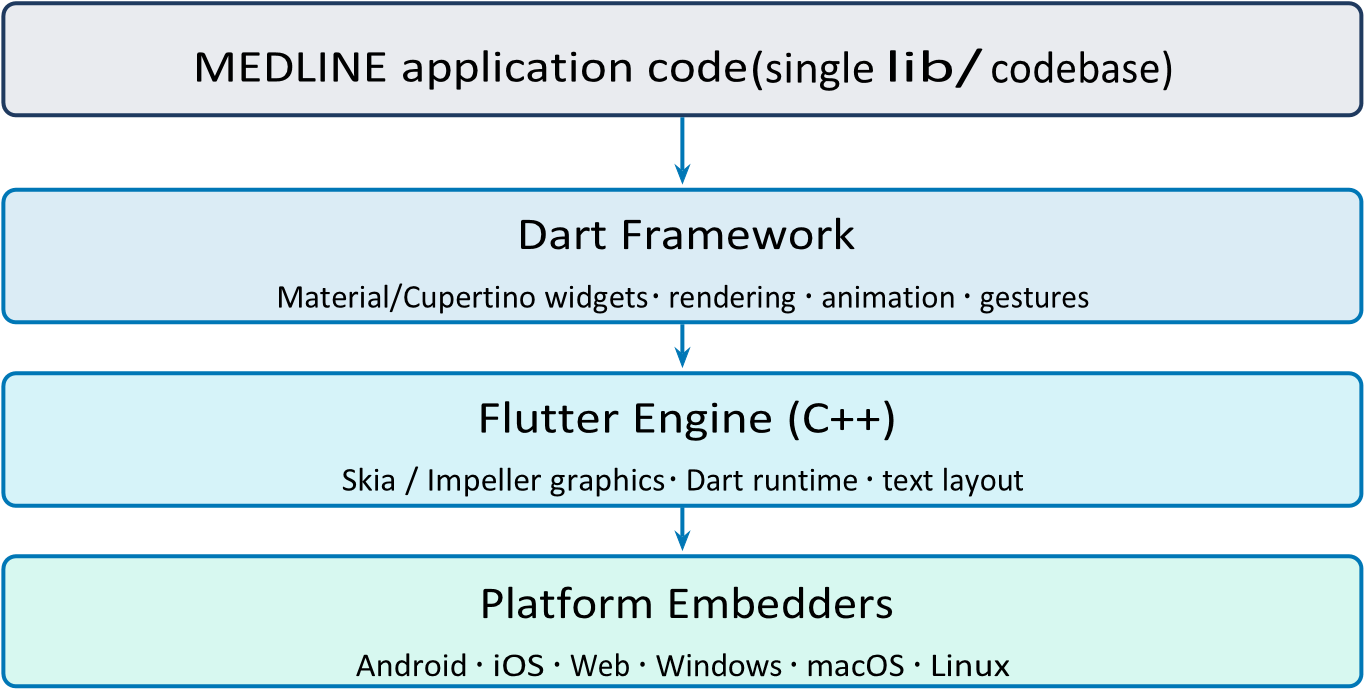
\includegraphics[width=0.85\textwidth]{fig1_1_flutter_arch.png}
  \caption{The layered Flutter architecture exploited by MEDLINE: one
           application codebase runs unchanged on every embedder.}
  \label{fig:flutter}
  \source{author-created illustration based on the Flutter architectural
          overview~\cite{flutterarch2024}.}
\end{figure}

\subsection{Dart Programming Language}

Dart is a strongly typed, ahead-of-time compiled language designed for
client-side development~\cite{dart2024}. Its \texttt{async}/\texttt{await}
syntax maps naturally to Firebase's asynchronous stream and future APIs. In
MEDLINE, \texttt{AuthWrapper} uses a \texttt{StreamBuilder} to listen to
Firebase Authentication state changes and a \texttt{FutureBuilder} to resolve
the Firestore user-role document --- both idiomatic Dart concurrency patterns
that keep the UI responsive during network operations.

\section{Role-Based Access Control (RBAC)}

Role-based access control is a security model in which permissions are assigned
to roles rather than directly to individual users~\cite{sandhu1996}. Sandhu et
al.\ formalised the RBAC96 model with four components: users, roles,
permissions, and sessions. Users are assigned to roles; roles are granted
permissions; sessions activate a subset of a user's assigned roles at
runtime~\cite{sandhu1996}.

Fernandez-Aleman et al.\ reviewed security mechanisms in electronic health
records and identified RBAC as the dominant access-control strategy in clinical
software, noting that improper access control is the leading cause of EHR data
breaches~\cite{fernandez2013}. MEDLINE implements a simplified RBAC96 subset:
six named roles (Table~\ref{tab:roles}) are stored per user in Firestore. The
\texttt{AuthWrapper} reads the authenticated user's role document and routes to
the corresponding dashboard, enforcing role isolation at the UI-routing layer.

\begin{table}[htbp]
  \centering
  \caption{MEDLINE user roles and primary responsibilities.}
  \label{tab:roles}
  \begin{tabularx}{\textwidth}{l X}
    \toprule
    \textbf{Role} & \textbf{Primary responsibilities}\\
    \midrule
    Admin & Monitor clinic-wide statistics, manage user accounts and role
            assignment, export administrative PDF reports.\\
    Receptionist & Search and register patients, schedule appointments, record
            payment method.\\
    Doctor & Review the daily patient queue, write consultation notes, assign
            diagnosis codes, issue referrals.\\
    Laboratory & Process diagnostic referrals, enter and complete test results,
            generate result sheets.\\
    Pharmacy & View prescriptions, confirm dispensing, flag out-of-stock items.\\
    Hospitalization & Assign beds, monitor inpatient daily status, record
            discharge.\\
    \bottomrule
  \end{tabularx}
  \source{author, derived from the implemented role routing in
          \texttt{auth\_wrapper.dart}.}
\end{table}

\section{Cloud Firestore and NoSQL Architecture}

NoSQL databases abandon the relational table model in favour of flexible
document, key-value, column-family, or graph structures~\cite{sadalage2013}.
Cloud Firestore is a document-oriented NoSQL database offered as part of Google
Firebase~\cite{firestore2024}. Data is organised into collections of documents
--- JSON-like key-value maps that can contain nested sub-collections.
Firestore's real-time snapshot listeners push incremental updates to connected
clients without polling, a property exploited in all MEDLINE dashboard widgets
via \texttt{StreamBuilder}.

Key Firestore characteristics relevant to MEDLINE are: offline persistence
(a local cache survives connectivity loss, critical in clinics with unstable
internet), security rules (server-side enforcement of read/write permissions by
authenticated UID), and composite-index support for multi-field queries such as
filtering patients by registration date and department~\cite{firestore2024}.

\section{State Management with Provider}

State management is a central architectural concern in Flutter: the framework
rebuilds widget subtrees on state change, so uncontrolled propagation causes
redundant rebuilds and tangled data flows~\cite{windmill2020}. The Provider
package wraps Flutter's \texttt{InheritedWidget} into a dependency-injection
container that notifies registered listeners on state
mutation~\cite{provider2024}.

MEDLINE uses two global providers. \texttt{ThemeProvider} manages
light/dark-mode preferences persisted via \texttt{SharedPreferences}, exposing
derived colour properties (\texttt{cardBackground}, \texttt{inputFill},
\texttt{textPrimary}) so that screen widgets remain palette-agnostic.
\texttt{LanguageProvider} holds the active locale (UZB, ENG, RUS, or KYR) with
a translation map covering more than two hundred UI string keys. Both providers
are injected at the root via \texttt{MultiProvider} in \texttt{main.dart},
making them accessible anywhere in the widget tree without manual
prop-drilling.

\section{Clinical Decision Support and AI in Healthcare}

A clinical decision support system (CDSS) is software that links
patient-specific information to a structured medical knowledge base in order to
generate case-specific assessments or recommendations that assist clinical
reasoning~\cite{sutton2020}. Two broad CDSS paradigms are commonly
distinguished. \emph{Knowledge-based} systems apply curated rules and explicit
symptom--disease associations (the classical expert-system branch of artificial
intelligence); \emph{non-knowledge-based} systems instead learn statistical
patterns from data using machine-learning models~\cite{sutton2020}.
Knowledge-based systems remain widely used in resource-limited settings because
they are transparent, require no training data, and are inexpensive to deploy,
whereas machine-learning systems demand large labelled datasets and careful
validation before clinical use.

MEDLINE integrates a lightweight knowledge-based diagnostic decision-support
model. A curated knowledge base of thirty-one diseases --- each associated with
a characteristic symptom set and a recommended specialist --- drives a scoring
function that ranks candidate diagnoses for a selected combination of symptoms
(detailed in Section~\ref{sec:diagnostic}). This positions the engine as an
AI-assisted \emph{triage aid} that suggests likely conditions and the
appropriate specialist, rather than as an autonomous diagnostic authority; a
migration toward data-driven machine-learning models is identified as future
work (Section~\ref{sec:futurework}). The choice of a rule-based model is
consistent with the constraints of the target clinics, which lack the labelled
clinical datasets and computational infrastructure required to train and serve
machine-learning classifiers.

\section{Automated PDF Report Generation}

Automated document generation is a standard requirement in clinical settings
--- for discharge summaries, prescription records, and administrative reports.
The \texttt{pdf} Dart package allows programmatic construction of PDF pages
using a box model similar to Flutter's widget system~\cite{pdfpkg2024}. MEDLINE
uses this package together with \texttt{printing} to render and share reports
directly from the application without server-side processing, keeping all
patient data on-device during rendering --- a privacy advantage in healthcare
contexts.

\section{Justification of Technology Choices}

The selection of Flutter over React Native is justified by its superior
rendering performance in benchmark comparisons~\cite{nawrocki2021}, a single
codebase for Android, iOS, and Web deployment, and strong support for custom UI
components --- important for the role-specific dashboard designs in MEDLINE.
Firebase was chosen over a self-hosted backend because the target clinics lack
dedicated IT infrastructure; Firestore's real-time listeners replace polling
and reduce complexity~\cite{firebase2024}. The Provider package was chosen over
Bloc or Riverpod because of its minimal boilerplate and sufficient capability
for the two global state concerns (theme and language) that MEDLINE
requires~\cite{provider2024}. Client-side PDF generation was preferred over
server-side rendering to eliminate a backend dependency and keep the system
fully serverless. Finally, a knowledge-based diagnostic model was preferred
over a machine-learning classifier because it is transparent and deployable
without training data~\cite{sutton2020}.

\section{Chapter Summary}

This chapter established the theoretical foundations underpinning MEDLINE.
Healthcare information systems provide the clinical and administrative context;
Flutter justifies the single-codebase cross-platform strategy; RBAC96 grounds
the six-role security model; Firestore's real-time document model supports the
live dashboard architecture; the Provider pattern organises global application
state; and knowledge-based clinical decision support frames the
symptom-matching diagnostic engine. Each technology choice was explicitly
justified against the project constraints. These foundations motivate the
requirements analysis in Chapter~2 and the design decisions described in
Chapter~3.

%============================== CHAPTER 2 =====================================
\chapter{Problem Domain Analysis and System Requirements}

This chapter analyses the operational environment that MEDLINE targets,
catalogues the deficiencies of current clinic workflows, identifies the
stakeholders, and derives the functional and non-functional requirements that
drive the design in Chapter~3.

\section{Target Environment Characteristics}

MEDLINE targets small and medium-sized private clinics operating multiple
service departments under a single administrative umbrella. A typical such
facility processes between fifty and three hundred patient visits per day
across departments including general consultation, laboratory diagnostics,
in-patient care, and pharmacy. The defining operational characteristic is the
need for cross-departmental data visibility: a receptionist registers a
patient; a doctor creates a referral; a laboratory technician uploads results;
a pharmacist dispenses medication --- all events must be traceable to a single
patient record in real time.

Prior to MEDLINE, clinics in this category typically employed one or more of:
paper ledgers and handwritten patient cards; general-purpose spreadsheet
software maintained independently per department; or disconnected desktop
billing software without clinical-data integration. Each approach introduces
distinct failure modes analysed in Section~\ref{sec:painpoints}.

\section{Operational Pain Points}
\label{sec:painpoints}

Table~\ref{tab:painpoints} catalogues the principal problems observed in manual
and semi-digital clinic workflows that directly informed the MEDLINE
requirements.

\begin{table}[htbp]
  \centering
  \caption{Operational pain points in manual and fragmented clinic workflows.}
  \label{tab:painpoints}
  \begin{tabularx}{\textwidth}{L{5cm} X}
    \toprule
    \textbf{Pain point} & \textbf{Consequence}\\
    \midrule
    Paper ledgers and handwritten cards & Illegible or lost records; no search;
      large physical storage requirement.\\
    Independent per-department spreadsheets & No single source of truth;
      cross-department data inconsistency and duplication.\\
    Disconnected billing software & Financial records cannot be reconciled with
      clinical activity; weak auditability.\\
    Manual report compilation & Daily, monthly, and yearly reports are slow to
      produce and error-prone.\\
    No real-time patient queue & Doctors are unaware of newly registered and
      waiting patients; consultation delays.\\
    No automated backup or access control & Risk of data loss and uncontrolled
      access to sensitive patient information.\\
    \bottomrule
  \end{tabularx}
  \source{author, based on analysis of the target clinic environment.}
\end{table}

\section{Stakeholder Analysis}

Six stakeholder groups were identified, each corresponding to one MEDLINE role.
Each group interacts with the system through a dedicated dashboard exposing only
the data and actions relevant to that role, as summarised in
Figure~\ref{fig:stakeholders}.

The \emph{receptionist} is the entry point of every patient journey, with the
primary use cases of searching existing patients, registering new patients with
demographic data, scheduling appointments, and recording the payment method.
The \emph{doctor} consults registered patients: viewing the assigned day queue,
writing consultation notes with ICD-10 diagnosis codes, issuing referrals to
laboratory or pharmacy, and reviewing visit history. The \emph{laboratory}
technician processes diagnostic referrals: viewing pending test requests,
entering quantitative or qualitative results, marking results as ready, and
generating PDF result sheets. The \emph{pharmacy} staff manage medication
dispensing: viewing incoming prescriptions, confirming dispensing, recording
stock deductions, and flagging out-of-stock items. The \emph{hospitalization}
department manages inpatient care: assigning patients to beds, monitoring daily
status, and recording discharge. Finally, the \emph{admin} monitors the entire
clinic: viewing real-time aggregate statistics, managing user accounts and role
assignments, and exporting administrative PDF reports.

\begin{figure}[htbp]
  \centering
  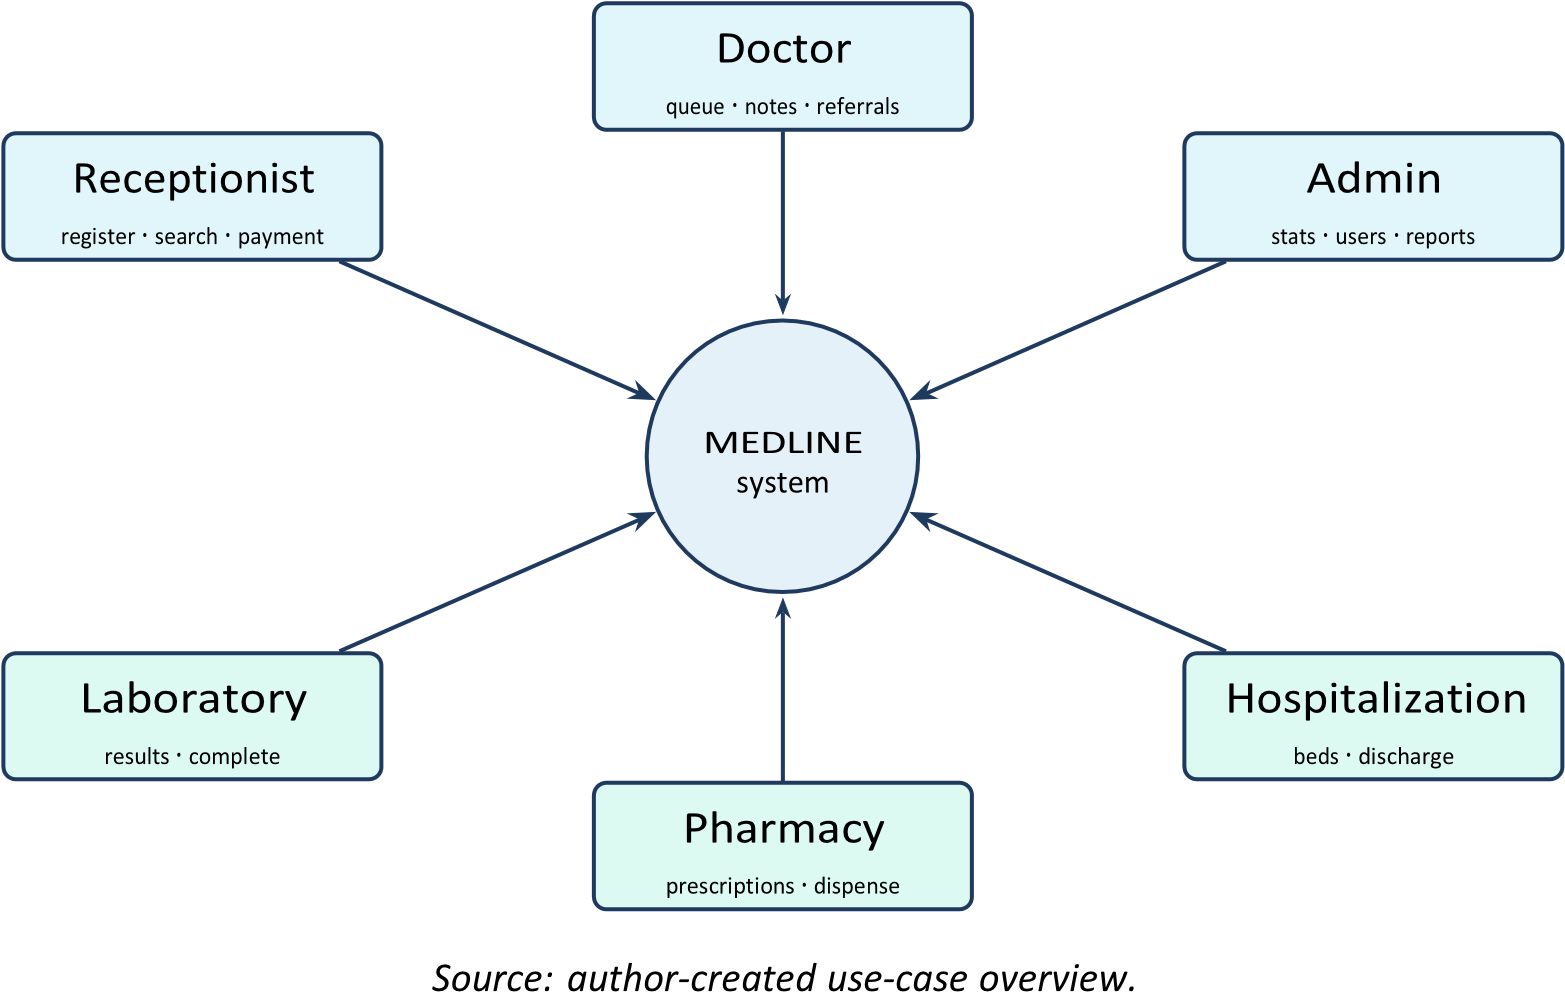
\includegraphics[width=0.9\textwidth]{fig2_1_stakeholders.png}
  \caption{Stakeholder--role overview: six actors interact with MEDLINE, each
           through a dedicated role dashboard.}
  \label{fig:stakeholders}
\end{figure}

\section{Functional Requirements}

Based on the stakeholder analysis and the observed workflow problems, the
functional requirements in Table~\ref{tab:fr} were defined for MEDLINE
following standard requirements-engineering practice~\cite{sommerville2016}.

\begin{table}[htbp]
  \centering
  \caption{Functional requirements of the MEDLINE system.}
  \label{tab:fr}
  \begin{tabularx}{\textwidth}{l X}
    \toprule
    \textbf{ID} & \textbf{Requirement}\\
    \midrule
    FR-01 & Authenticate users via email and password and restrict access to
            role-specific views.\\
    FR-02 & Allow a receptionist to register a new patient with name, date of
            birth, gender, contact details, and visit purpose.\\
    FR-03 & Display a real-time patient queue on the doctor dashboard, updated
            without manual page refresh.\\
    FR-04 & Allow doctors to record consultation notes, assign an ICD-10
            diagnosis code, and issue referrals to laboratory or pharmacy.\\
    FR-05 & Allow laboratory staff to enter test results and mark requests as
            completed.\\
    FR-06 & Allow pharmacy staff to view prescriptions and confirm dispensing.\\
    FR-07 & Allow hospitalization staff to manage bed assignments and inpatient
            status updates.\\
    FR-08 & Display, on the admin dashboard, aggregated statistics filterable by
            today, this week, and this month.\\
    FR-09 & Generate PDF reports for patient records and administrative
            summaries.\\
    FR-10 & Support the user interface in four languages: Uzbek, English,
            Russian, and Kyrgyz.\\
    \bottomrule
  \end{tabularx}
  \source{author.}
\end{table}

\section{Non-Functional Requirements}

The non-functional requirements in Table~\ref{tab:nfr} constrain the quality
attributes of the system.

\begin{table}[htbp]
  \centering
  \caption{Non-functional requirements of the MEDLINE system.}
  \label{tab:nfr}
  \begin{tabularx}{\textwidth}{l l X}
    \toprule
    \textbf{ID} & \textbf{Category} & \textbf{Requirement}\\
    \midrule
    NFR-01 & Performance & Dashboard data shall load within 3 seconds on a
             standard LTE connection.\\
    NFR-02 & Availability & The system shall leverage Firebase managed
             infrastructure targeting 99.9\% uptime.\\
    NFR-03 & Security & Data at rest shall be protected by Firestore security
             rules; data in transit shall use TLS 1.2 or higher.\\
    NFR-04 & Usability & The interface shall conform to Material Design 3
             guidelines for intuitive navigation by non-technical clinical
             staff.\\
    NFR-05 & Portability & The application shall deploy without code
             modification on Android, iOS, and the Web.\\
    NFR-06 & Maintainability & Business logic shall be separated from the UI via
             Provider state management to facilitate future feature additions.\\
    \bottomrule
  \end{tabularx}
  \source{author.}
\end{table}

\section{Comparison with Existing Systems}

Table~\ref{tab:comparison} compares MEDLINE with representative alternatives to
contextualise its scope and positioning. Adebayo and Lim demonstrated the
feasibility of mobile-based patient management in resource-limited settings,
but confined their system to a single Android application without a shared
backend~\cite{adebayo2021}. OpenMRS, while comprehensive, requires a dedicated
server, a database administrator, and significant configuration effort ---
barriers that exceed the capacity of small private clinics. MEDLINE occupies a
distinct niche: serverless, cross-platform, zero-infrastructure-cost, with
real-time multi-role dashboards and automated PDF reporting in a single
codebase.

\begin{table}[htbp]
  \centering
  \caption{Comparison of MEDLINE with selected clinic-management approaches.}
  \label{tab:comparison}
  \small
  \begin{tabularx}{\textwidth}{L{3.6cm} c c c c}
    \toprule
    \textbf{Criterion} & \textbf{MEDLINE} & \textbf{OpenMRS} &
      \textbf{Mobile app~\cite{adebayo2021}} & \textbf{Spreadsheets}\\
    \midrule
    Cross-platform & Android/iOS/Web & Web only & Android only & Partial\\
    Real-time multi-role dashboards & Yes & No & Yes & No\\
    Automated PDF reporting & Yes & Partial & Yes & No\\
    Serverless / zero-infrastructure & Yes & No & Partial & Yes\\
    Diagnostic decision support & Yes & Plugin & No & No\\
    Licensing / infrastructure cost & None & High & Low & Low\\
    \bottomrule
  \end{tabularx}
  \source{author's comparative analysis.}
\end{table}

\section{Sub-Conclusions}

The analysis reveals that small private clinics face a concrete set of
operational deficiencies rooted in paper-based or fragmented digital workflows.
Six stakeholder groups generate ten functional and six non-functional
requirements. Comparison with existing systems confirms that no widely
available solution combines a serverless cloud backend, real-time multi-role
dashboards, automated PDF reporting, a built-in diagnostic aid, and
cross-platform deployment at zero licensing cost. These findings motivate the
design and implementation described in Chapter~3.

%============================== CHAPTER 3 =====================================
\chapter{System Design and Implementation}

This chapter documents how the requirements established in Chapter~2 were
realised in the MEDLINE system. It describes the layered architecture, the
Firebase backend, the structure of the Flutter client, the six role-specific
dashboards, the multilingual and theming subsystems, the automated PDF
reporting pipeline, and the rule-based diagnostic decision-support module that
gives the system its analytical capability.

\section{System Architecture Overview}

MEDLINE follows a client--server architecture in which the client is a Flutter
application and the server tier is entirely managed by Google Firebase. This
serverless model eliminates the need for a dedicated backend server, reduces
operational overhead, and leverages Firebase's built-in horizontal
scaling~\cite{firebase2024}. The system is organised into five logical layers,
shown in Figure~\ref{fig:fivelayer}, each with a clearly delimited
responsibility:

\begin{itemize}
  \item \textbf{Presentation layer} --- the Flutter widget tree rendering
        role-specific dashboards and shared UI components.
  \item \textbf{State-management layer} --- Provider \texttt{ChangeNotifier}
        classes (\texttt{ThemeProvider}, \texttt{LanguageProvider}) that
        broadcast state changes to the widget tree~\cite{provider2024}.
  \item \textbf{Authentication layer} --- Firebase Authentication managing
        email/password verification, password-reset flows, and JWT session
        persistence~\cite{firebaseauth2024}.
  \item \textbf{Data layer} --- Cloud Firestore storing patient records, user
        profiles, departmental events, and financial transactions as JSON
        documents~\cite{firestore2024}.
  \item \textbf{Services layer} --- the \texttt{pdf} and \texttt{printing}
        packages for client-side report generation and \texttt{webview\_flutter}
        for embedded diagnostic web content.
\end{itemize}

The boundary between the data layer and the layers above it is the Firebase
network API; everything from the authentication layer upward executes on the
client device. This separation is what allows a single Flutter codebase to be
compiled for Android, iOS, and the Web without server-side components.

\begin{figure}[htbp]
  \centering
  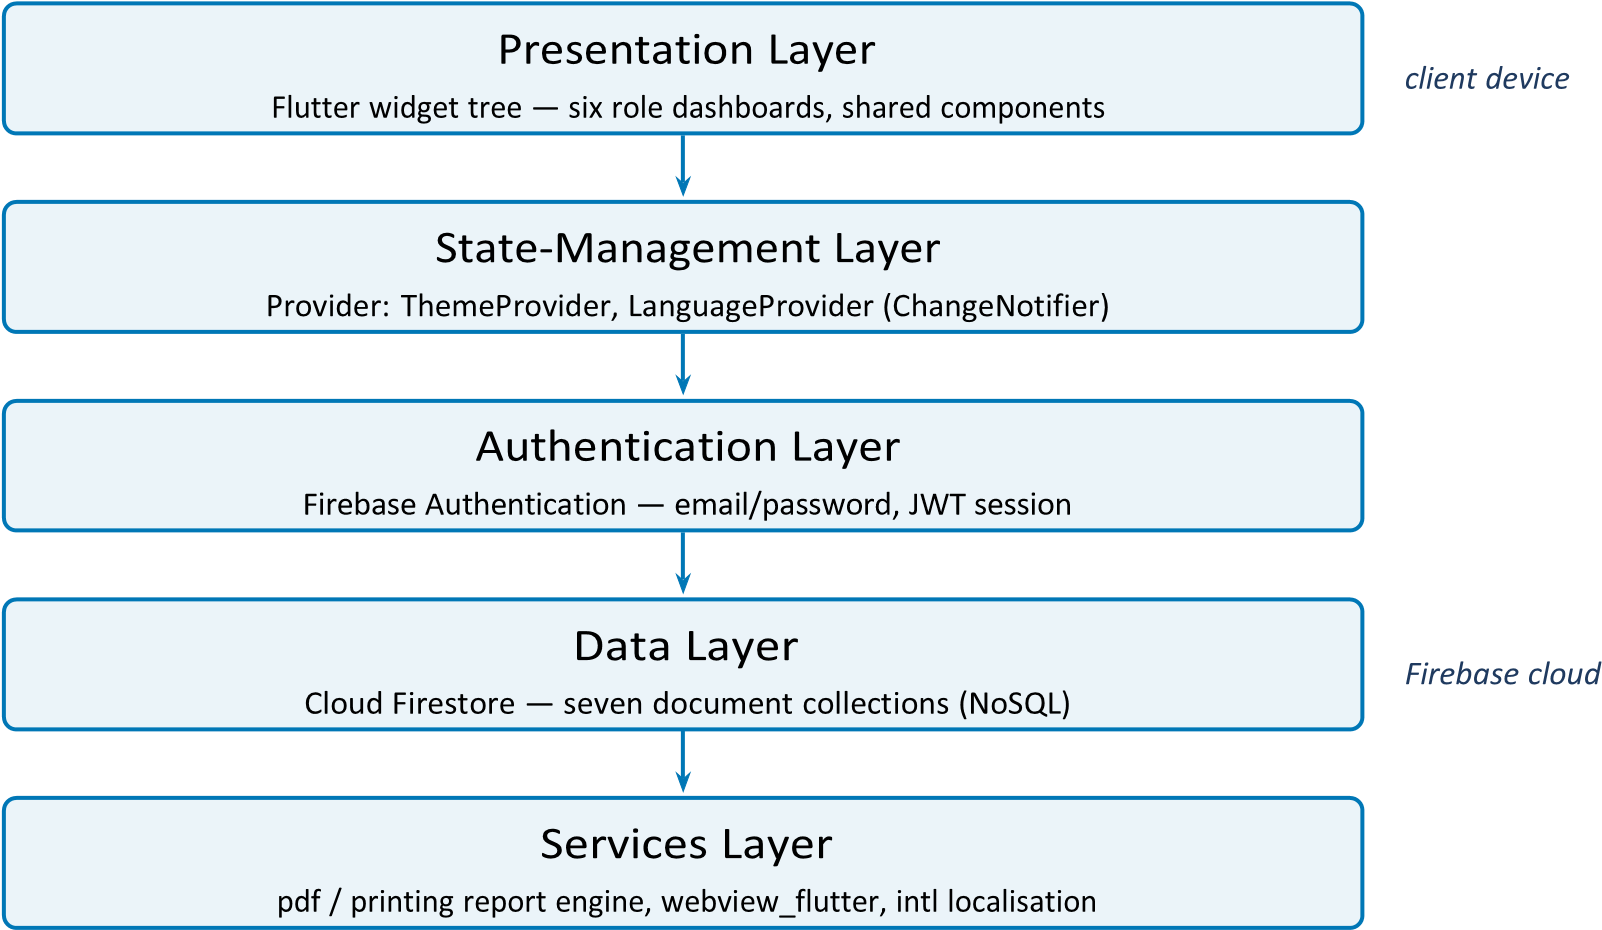
\includegraphics[width=0.85\textwidth]{fig3_1_five_layer.png}
  \caption{Five-layer architecture of the MEDLINE clinic-management system.}
  \label{fig:fivelayer}
  \source{author, derived from the MEDLINE source tree.}
\end{figure}

\section{Firebase Backend Design}

\subsection{Firestore Data Model}

Firestore organises MEDLINE data into seven top-level collections. Each
collection stores a specific entity type as independent JSON documents
addressable by an auto-generated or UID-based key~\cite{sadalage2013}.
Table~\ref{tab:collections} summarises the collections and their principal
fields; Figure~\ref{fig:firestore} depicts the document-oriented model
graphically.

Because Firestore is a NoSQL document store, there are no enforced foreign keys;
relationships such as the link between a \texttt{lab\_requests} document and its
\texttt{patients} document are maintained at the application level through the
stored \texttt{patientId} field. This denormalised design favours fast,
single-collection reads --- the dominant access pattern for the real-time
dashboards --- over relational integrity guarantees~\cite{sadalage2013}.

\begin{table}[htbp]
  \centering
  \caption{Firestore collections and key document fields.}
  \label{tab:collections}
  \begin{tabularx}{\textwidth}{l L{4cm} X}
    \toprule
    \textbf{Collection} & \textbf{Purpose} & \textbf{Key fields}\\
    \midrule
    \texttt{users} & Staff accounts and roles &
      \texttt{uid, email, fullName, role, createdAt}\\
    \texttt{patients} & Patient demographic records &
      \texttt{fullName, phone, gender, birthDate, registeredAt}\\
    \texttt{lab\_requests} & Laboratory test orders &
      \texttt{patientId, testType, status, result, completedAt}\\
    \texttt{prescriptions} & Medication prescriptions &
      \texttt{patientId, doctorId, drug, dosage, dispensed}\\
    \texttt{payments} & Financial transactions &
      \texttt{patientId, amount, type, timestamp}\\
    \texttt{events} & Departmental scheduling items &
      \texttt{title, department, start, end}\\
    \texttt{beds} & Hospitalization bed status &
      \texttt{bedNo, patientId, status, admittedAt}\\
    \bottomrule
  \end{tabularx}
  \source{author, extracted from Firestore queries in the MEDLINE codebase.}
\end{table}

\begin{figure}[htbp]
  \centering
  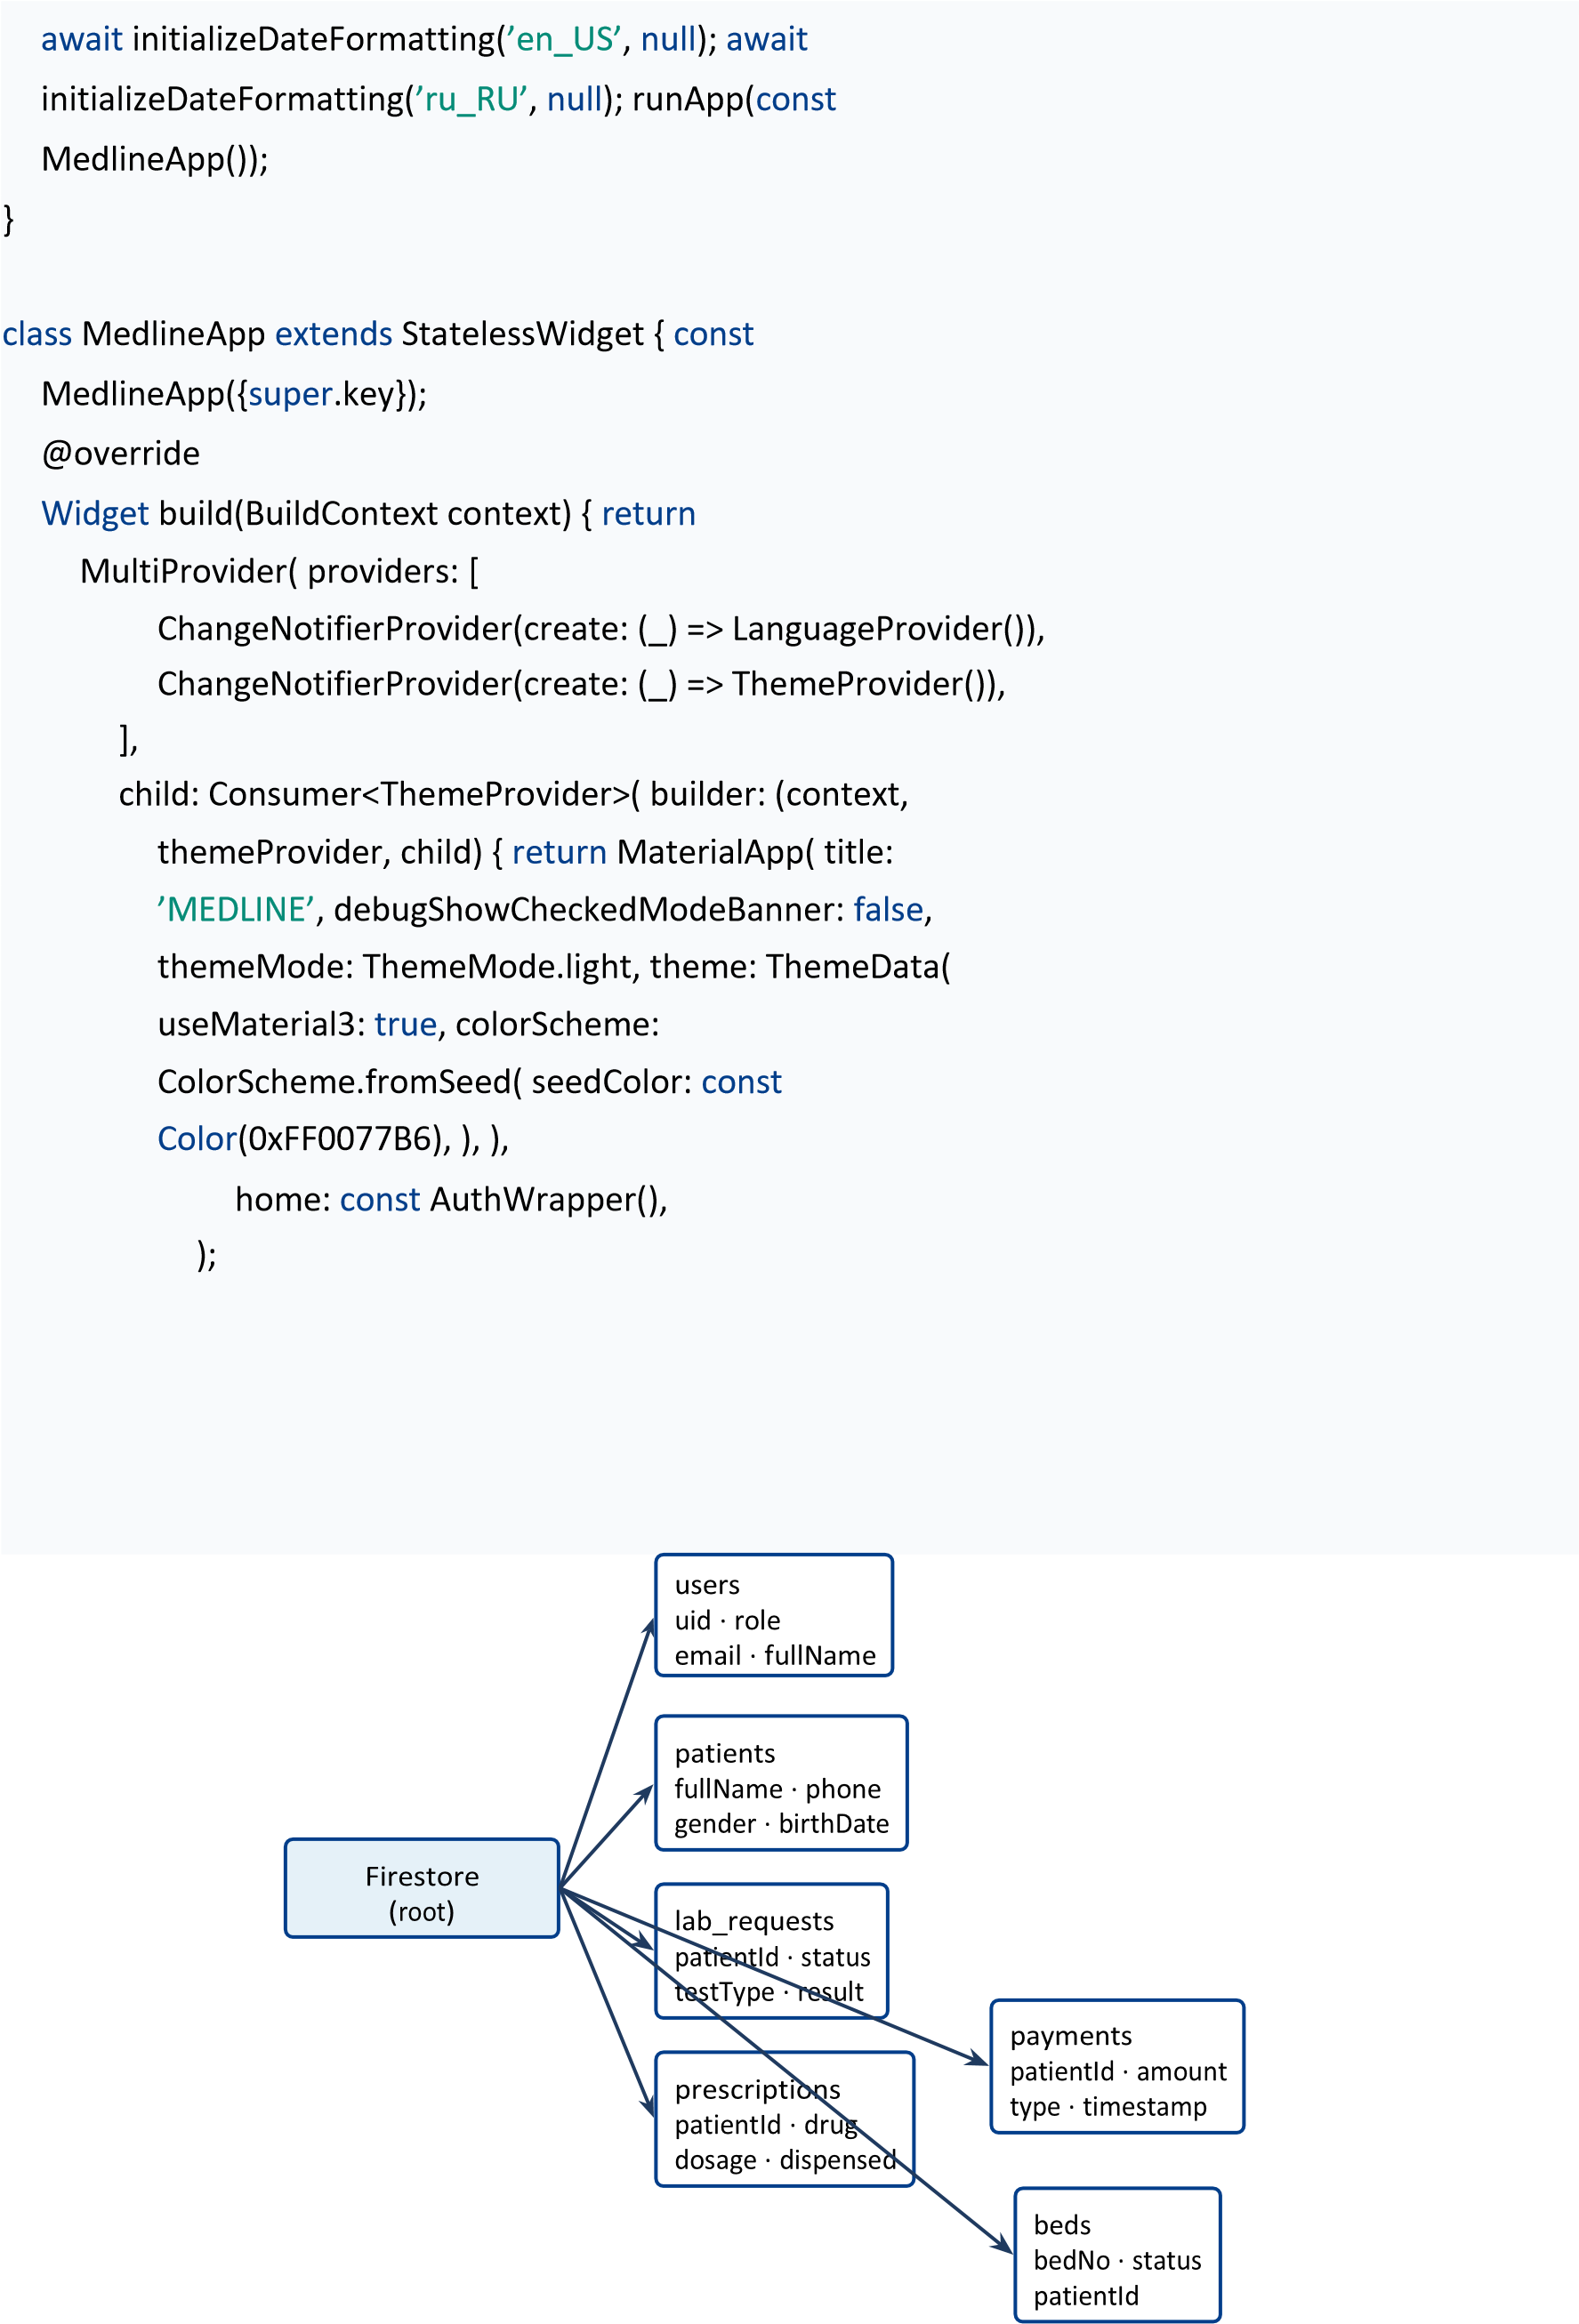
\includegraphics[width=0.85\textwidth]{fig3_2_firestore_model.png}
  \caption{Document-oriented Firestore data model with seven top-level
           collections.}
  \label{fig:firestore}
  \source{author. Logical references between collections (e.g.\
          \texttt{patientId}) are enforced at the application level.}
\end{figure}

\subsection{Authentication and Role Routing}

Firebase Authentication issues a JSON Web Token (JWT) on successful login. The
token UID is used as the document key in the \texttt{users} collection, binding
every authenticated session to exactly one role record. The
\texttt{AuthWrapper} widget (in \texttt{lib/auth/auth\_wrapper.dart}) implements
the role-routing procedure given in Algorithm~\ref{alg:authwrapper}.

Critically, new users are created only by the Admin through the Register screen;
the \texttt{role} field is written to Firestore at registration time and is
never modifiable by the end user. Because the destination dashboard route is
selected from the server-stored role rather than from any client-held value,
privilege escalation through the client is structurally impossible --- a direct
application of the RBAC principle discussed in Chapter~1~\cite{sandhu1996}. The
Flutter entry point that bootstraps this flow is shown in
Listing~\ref{lst:main}.

\begin{algorithm}[htbp]
  \caption{\texttt{AuthWrapper} authentication and role routing}
  \label{alg:authwrapper}
  \begin{algorithmic}[1]
    \State Subscribe to \textsc{FirebaseAuth.authStateChanges()} stream
    \If{stream state $=$ \emph{waiting}}
      \State render loading indicator
    \ElsIf{no authenticated user}
      \State navigate to \textsc{LoginScreen}
    \Else
      \State $uid \gets$ authenticated user UID
      \State $doc \gets$ \textsc{Firestore}.collection(\texttt{users}).doc($uid$).get()
      \If{$doc$ does not exist}
        \State show error; offer logout
      \Else
        \State $role \gets doc.\text{data()}[\texttt{role}]$
        \State navigate to dashboard widget corresponding to $role$
      \EndIf
    \EndIf
  \end{algorithmic}
\end{algorithm}

\begin{lstlisting}[caption={Application bootstrap and provider wiring in
  \texttt{main.dart}.},label={lst:main}]
void main() async {
  WidgetsFlutterBinding.ensureInitialized();
  await Firebase.initializeApp(
    options: DefaultFirebaseOptions.currentPlatform,
  );
  await initializeDateFormatting('uz_UZ', null);
  runApp(
    MultiProvider(
      providers: [
        ChangeNotifierProvider(create: (_) => ThemeProvider()),
        ChangeNotifierProvider(create: (_) => LanguageProvider()),
      ],
      child: const MedlineApp(),
    ),
  );
}
\end{lstlisting}

\section{Flutter Application Structure}

The project follows a feature-first directory layout under \texttt{lib/}. The
\texttt{auth/} directory contains \texttt{AuthWrapper}; \texttt{screens/} holds
one Dart file per major screen or dashboard; \texttt{providers/} contains
\texttt{ThemeProvider} and \texttt{LanguageProvider}; \texttt{utils/} holds
shared utilities such as \texttt{AppDateUtils} and \texttt{CacheManager}; and
\texttt{theme/} holds the colour and style constants. The \texttt{main.dart}
entry point initialises Firebase, pre-loads locale data for three regions
(Uzbek, English, Russian), and mounts the widget tree wrapped in a
\texttt{MultiProvider}, as shown in Listing~\ref{lst:main}. This separation
keeps business logic in providers and utilities, isolated from the presentation
code in \texttt{screens/}, satisfying the maintainability requirement NFR-06.

\section{Role-Specific Dashboards}

Each of the six roles is served by a dedicated \texttt{StatefulWidget}
dashboard. All dashboards share a structural pattern: a gradient background with
floating particle decoration, an animated fade-in on mount via an
\texttt{AnimationController}, a \texttt{StreamBuilder} bound to a Firestore
query for real-time updates, and a \texttt{BottomNavigationBar} or tab structure
for subsection navigation. Table~\ref{tab:dashboards} maps each dashboard to its
primary Firestore data source.

\begin{figure}[htbp]
  \centering
  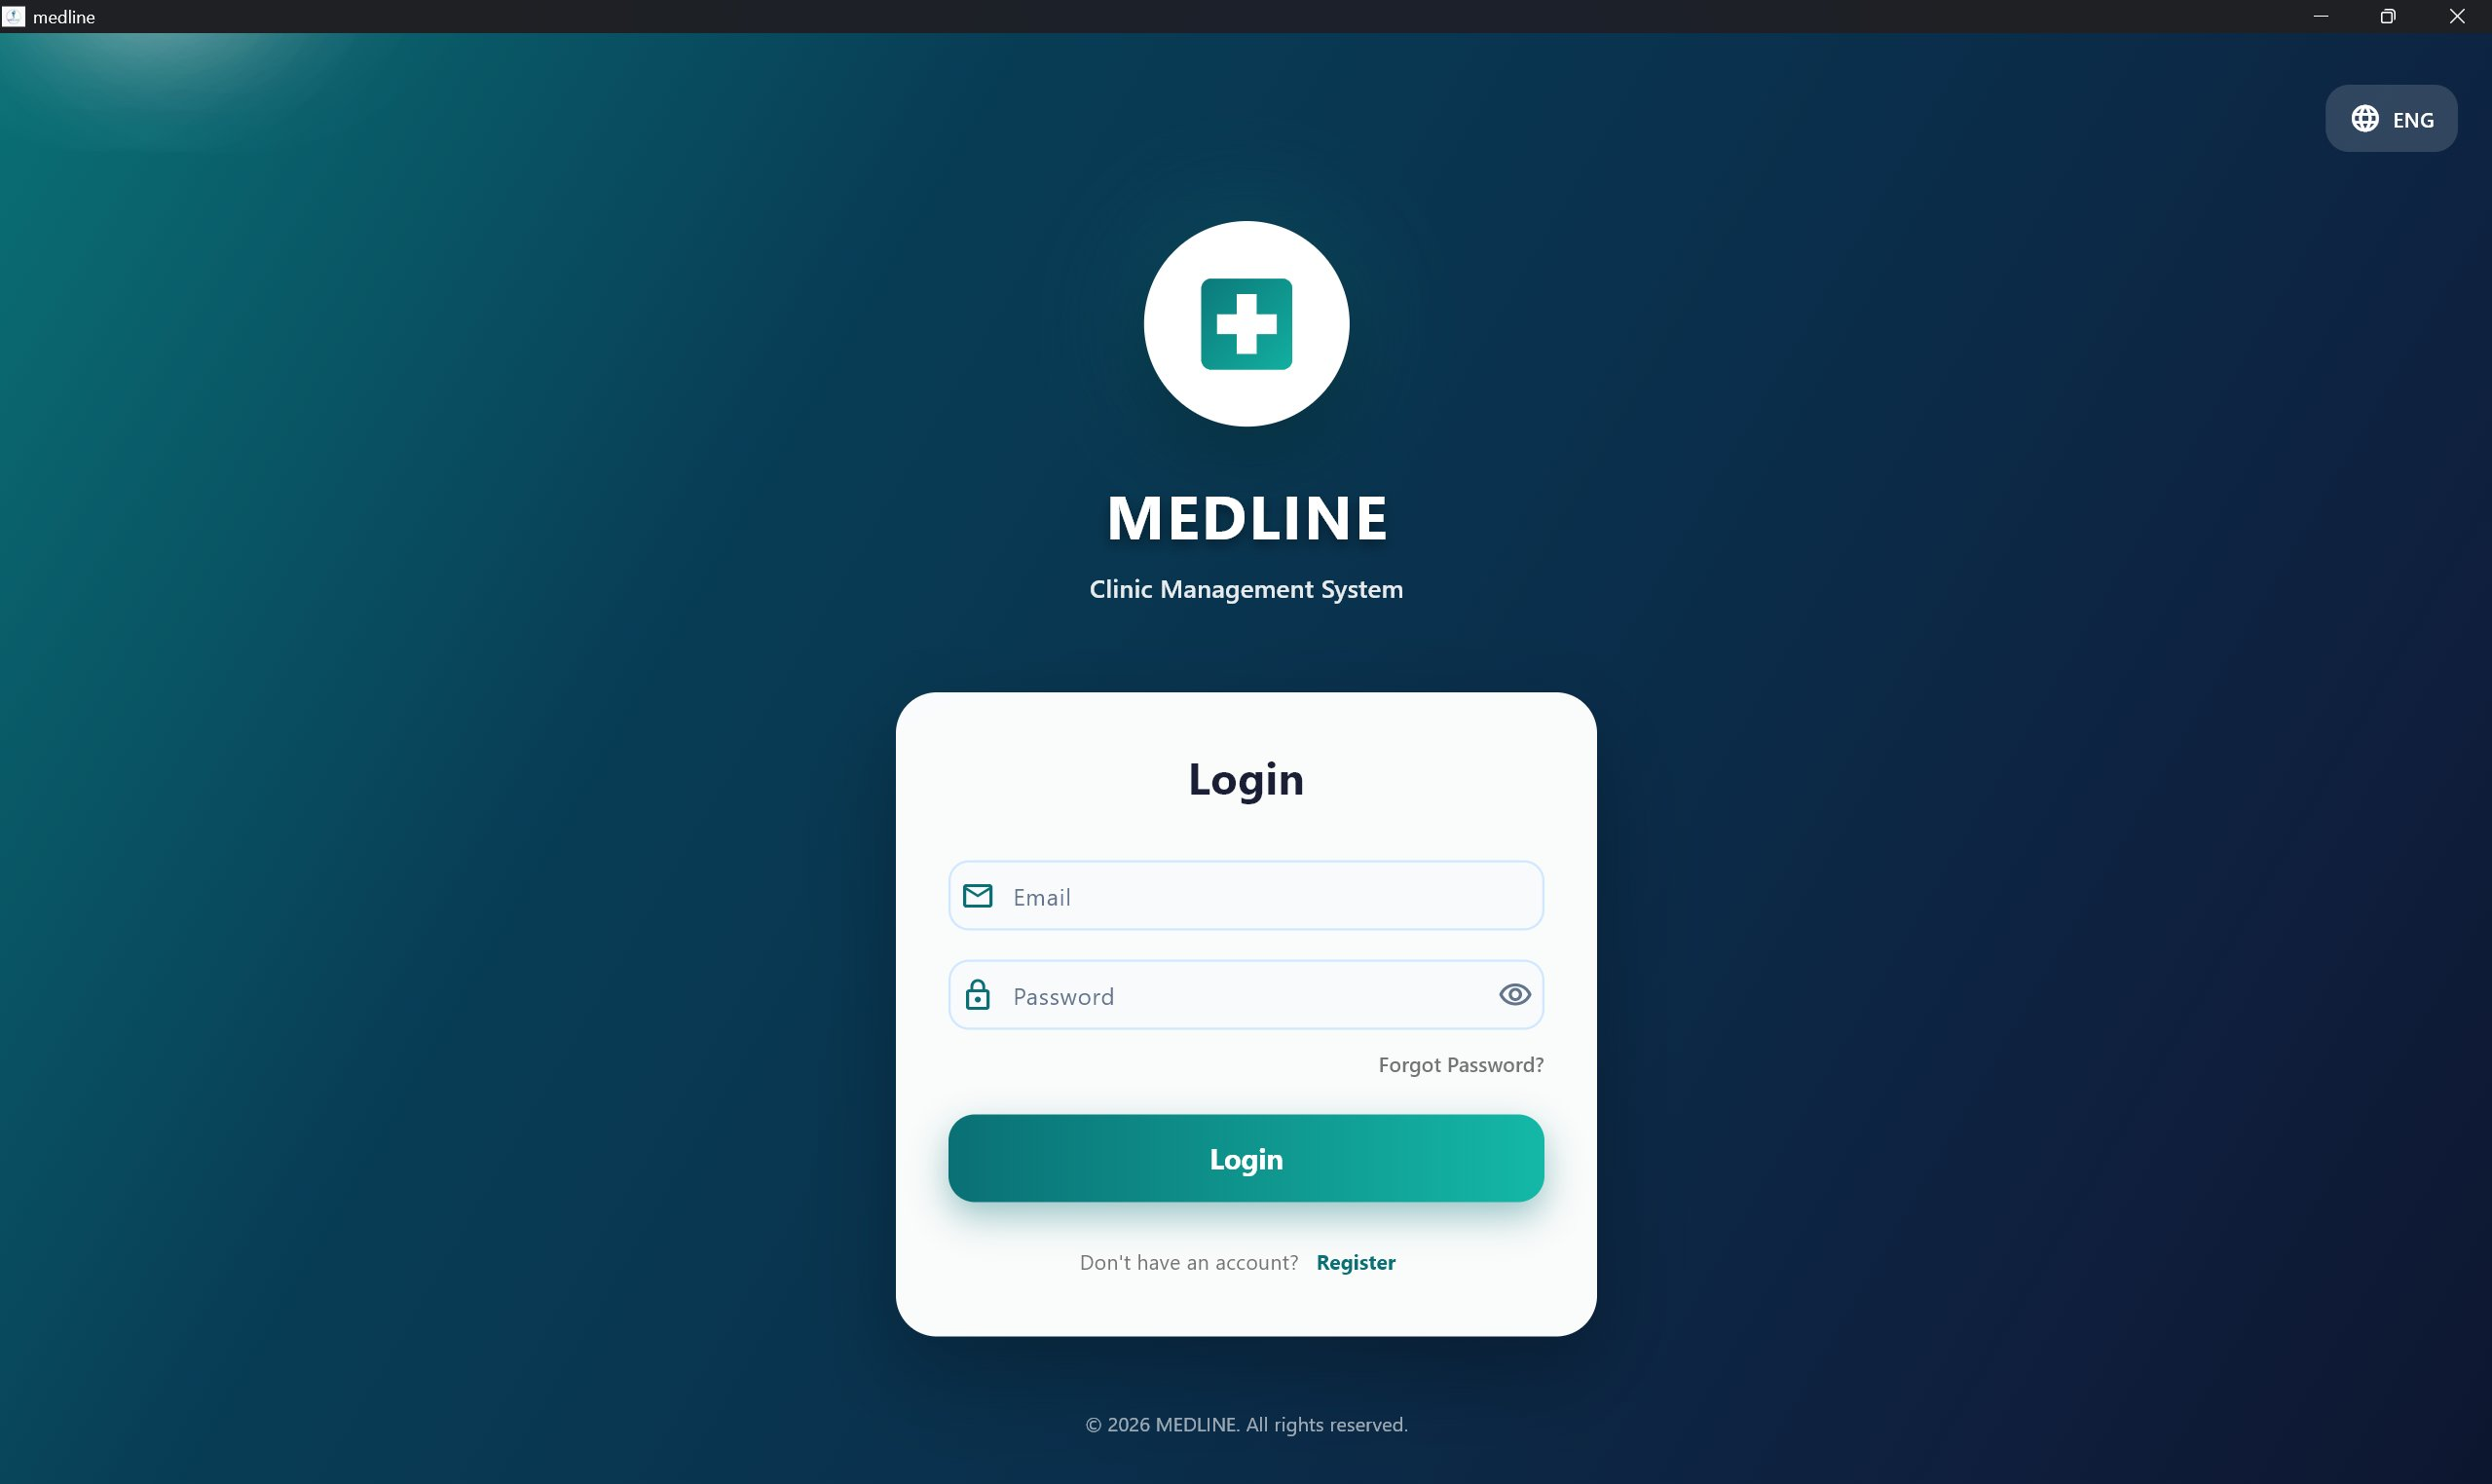
\includegraphics[width=0.45\textwidth]{fig3_4_login.png}
  \caption{MEDLINE login screen: the email and password authentication entry
           point with a language selector, rendered from the shared Flutter
           codebase.}
  \label{fig:login}
  \source{author's screenshot of the implemented MEDLINE application.}
\end{figure}

\begin{table}[htbp]
  \centering
  \caption{Role dashboards and primary Firestore data sources.}
  \label{tab:dashboards}
  \begin{tabularx}{\textwidth}{l L{4.5cm} X}
    \toprule
    \textbf{Dashboard} & \textbf{Collection(s)} &
      \textbf{Principal query / action}\\
    \midrule
    Admin & \texttt{payments}, \texttt{patients}, \texttt{users} &
      aggregate revenue and counts; manage roles\\
    Doctor & \texttt{patients}, \texttt{lab\_requests}, \texttt{prescriptions} &
      today's patients; write referrals\\
    Receptionist & \texttt{patients} &
      prefix search on \texttt{fullName}; register patient\\
    Laboratory & \texttt{lab\_requests} &
      stream \texttt{status == pending}; complete result\\
    Pharmacy & \texttt{prescriptions} & list incoming; mark dispensed\\
    Hospitalization & \texttt{beds}, \texttt{patients} &
      bed-status grid; admit / discharge\\
    \bottomrule
  \end{tabularx}
  \source{author.}
\end{table}

\subsection{Admin Dashboard}

The Admin dashboard fetches all payment and patient documents from Firestore and
aggregates them client-side into period-filtered statistics (today, this week,
this month). Revenue is formatted using the Uzbek number locale
(\texttt{NumberFormat('\#,\#\#\#', 'uz\_UZ')}). Three tabs are exposed: a
statistics overview, a full patient list with search, and a user-management
panel for role assignment.

\begin{figure}[htbp]
  \centering
  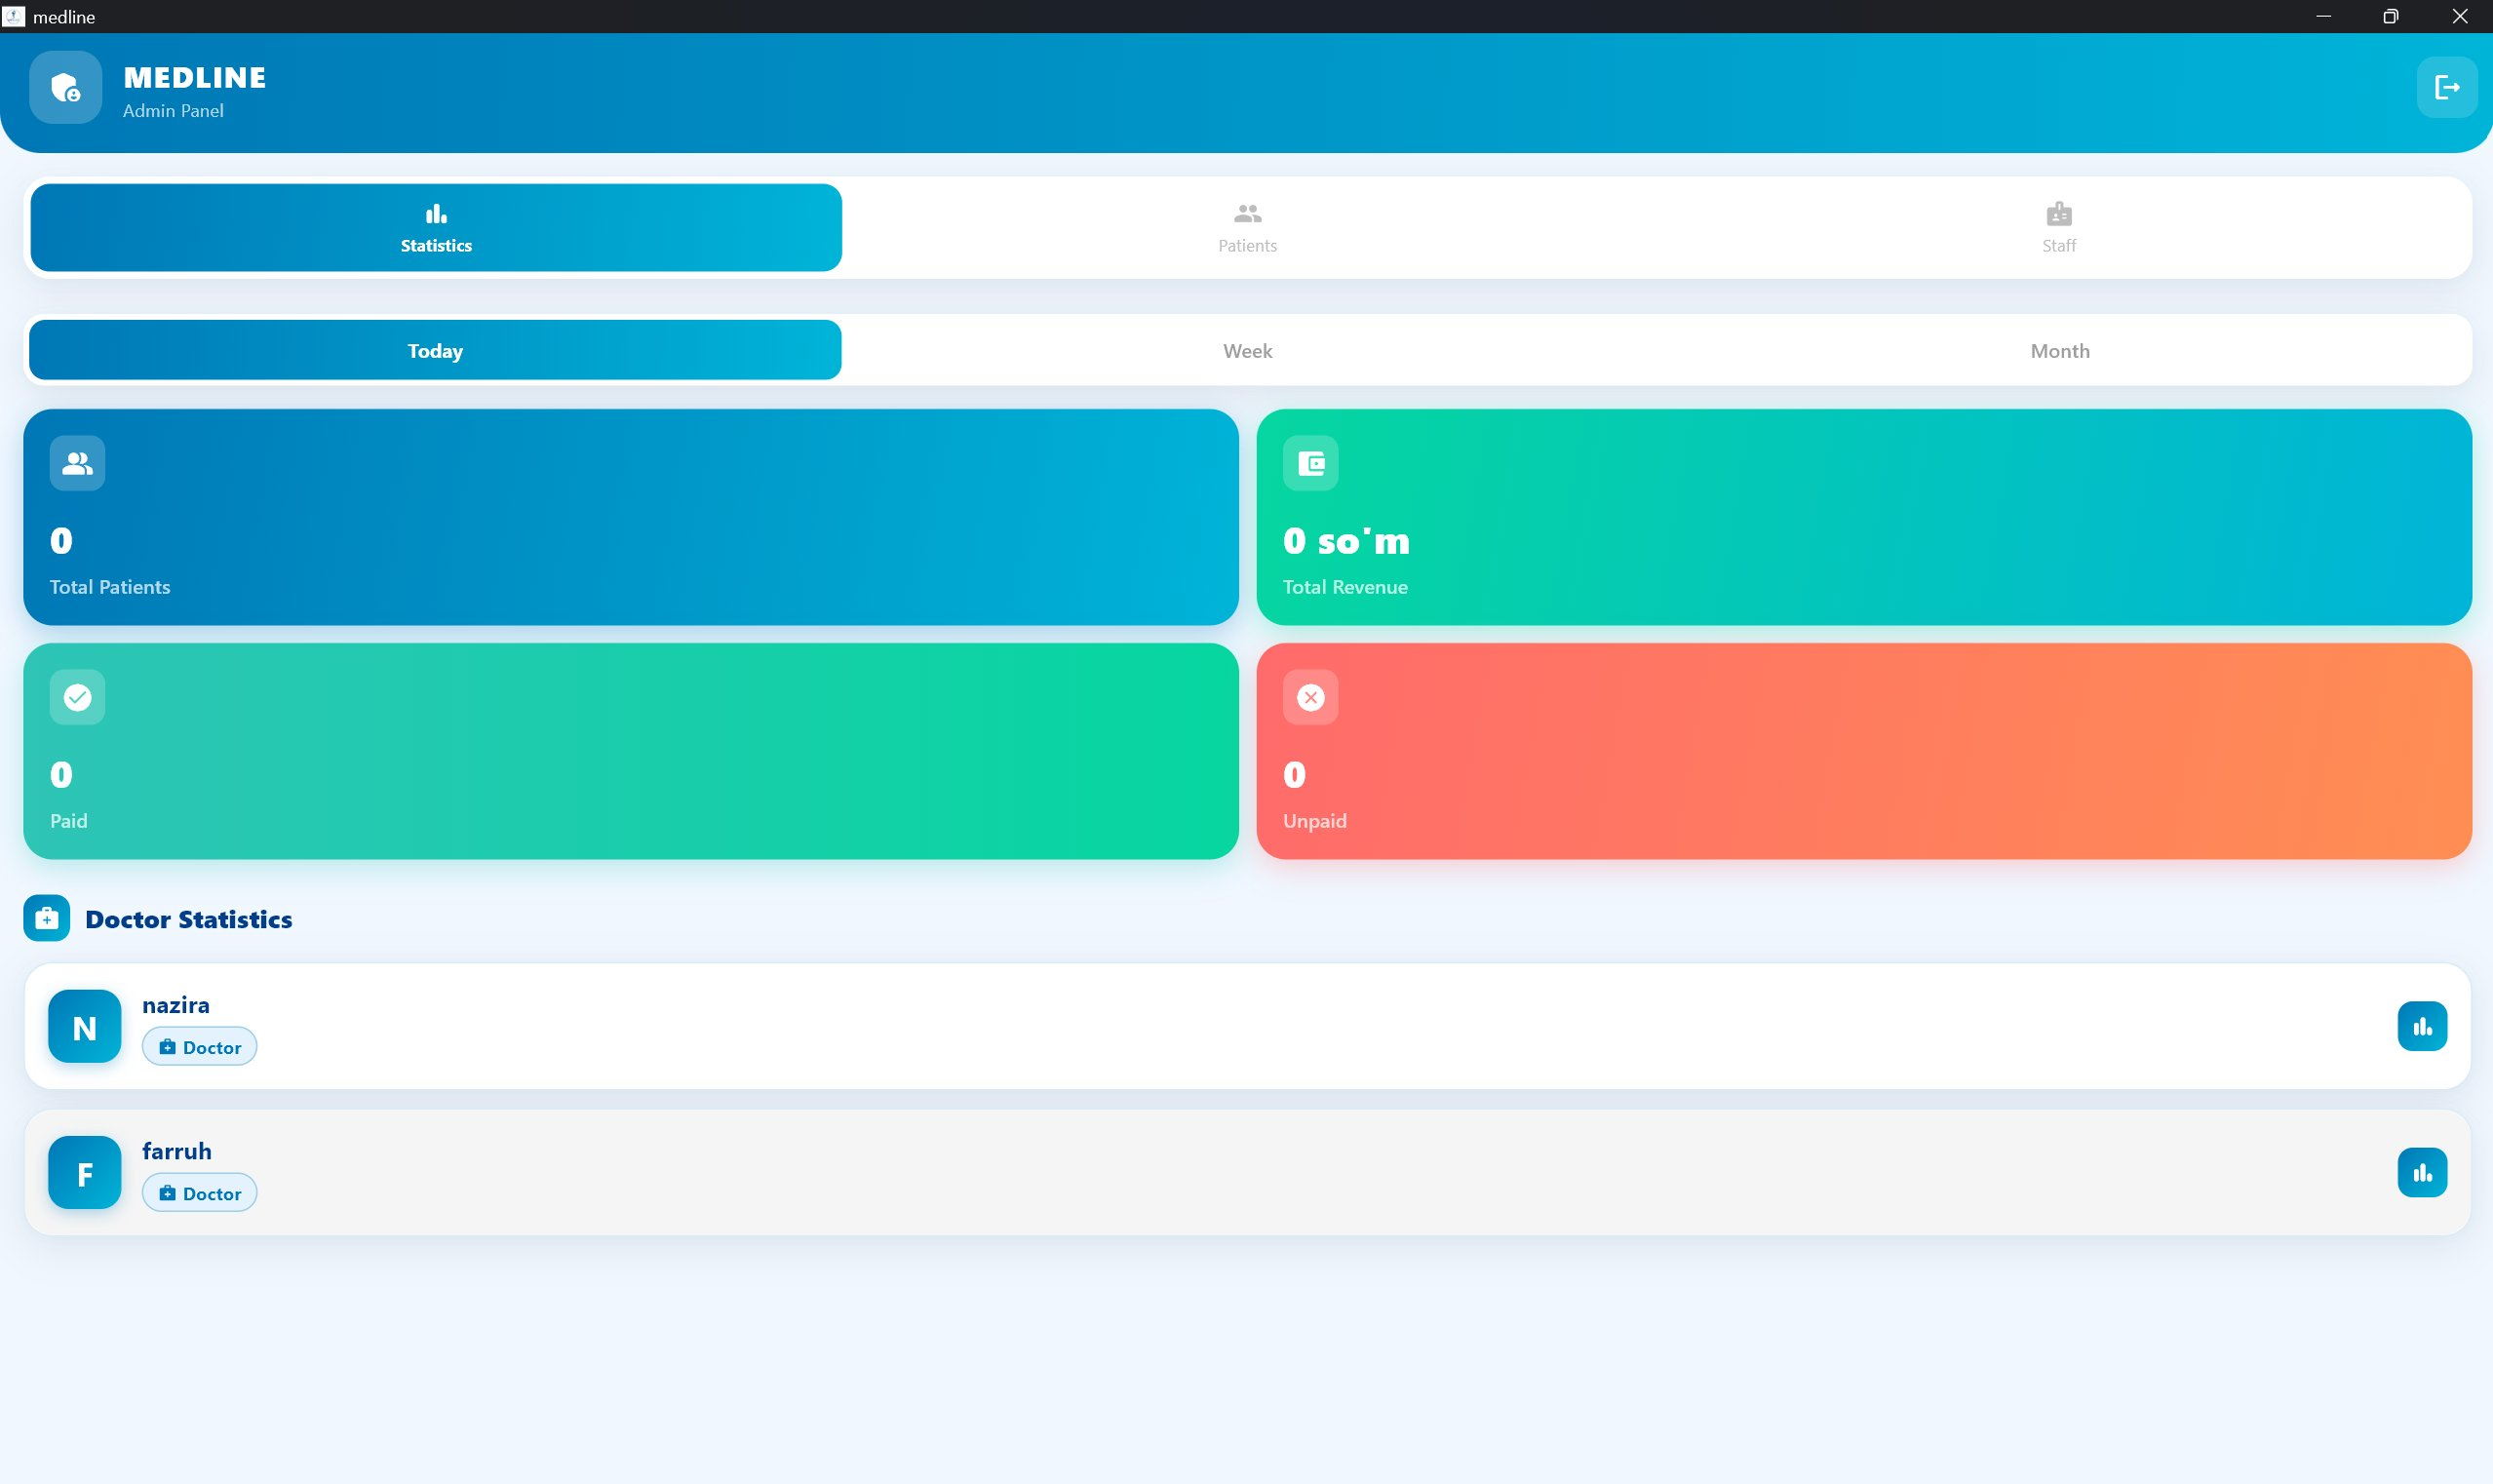
\includegraphics[width=0.8\textwidth]{fig3_5_admin.png}
  \caption{Admin dashboard: clinic-wide statistics showing total patients,
           total revenue, paid and unpaid counts, and per-doctor breakdowns with
           Today / Week / Month filters.}
  \label{fig:admin}
  \source{author's screenshot of the implemented MEDLINE application.}
\end{figure}

\subsection{Doctor Dashboard}

The Doctor dashboard queries Firestore for patients registered within the
current calendar day using a timestamp range filter. Each patient card is
expandable to enter a consultation note, assign an ICD-10 diagnosis code
(free-text in the current version), and dispatch referrals by writing to the
\texttt{lab\_requests} or \texttt{prescriptions} collections. Completed
consultations are stored with the doctor's UID and a server-side timestamp.

\begin{figure}[htbp]
  \centering
  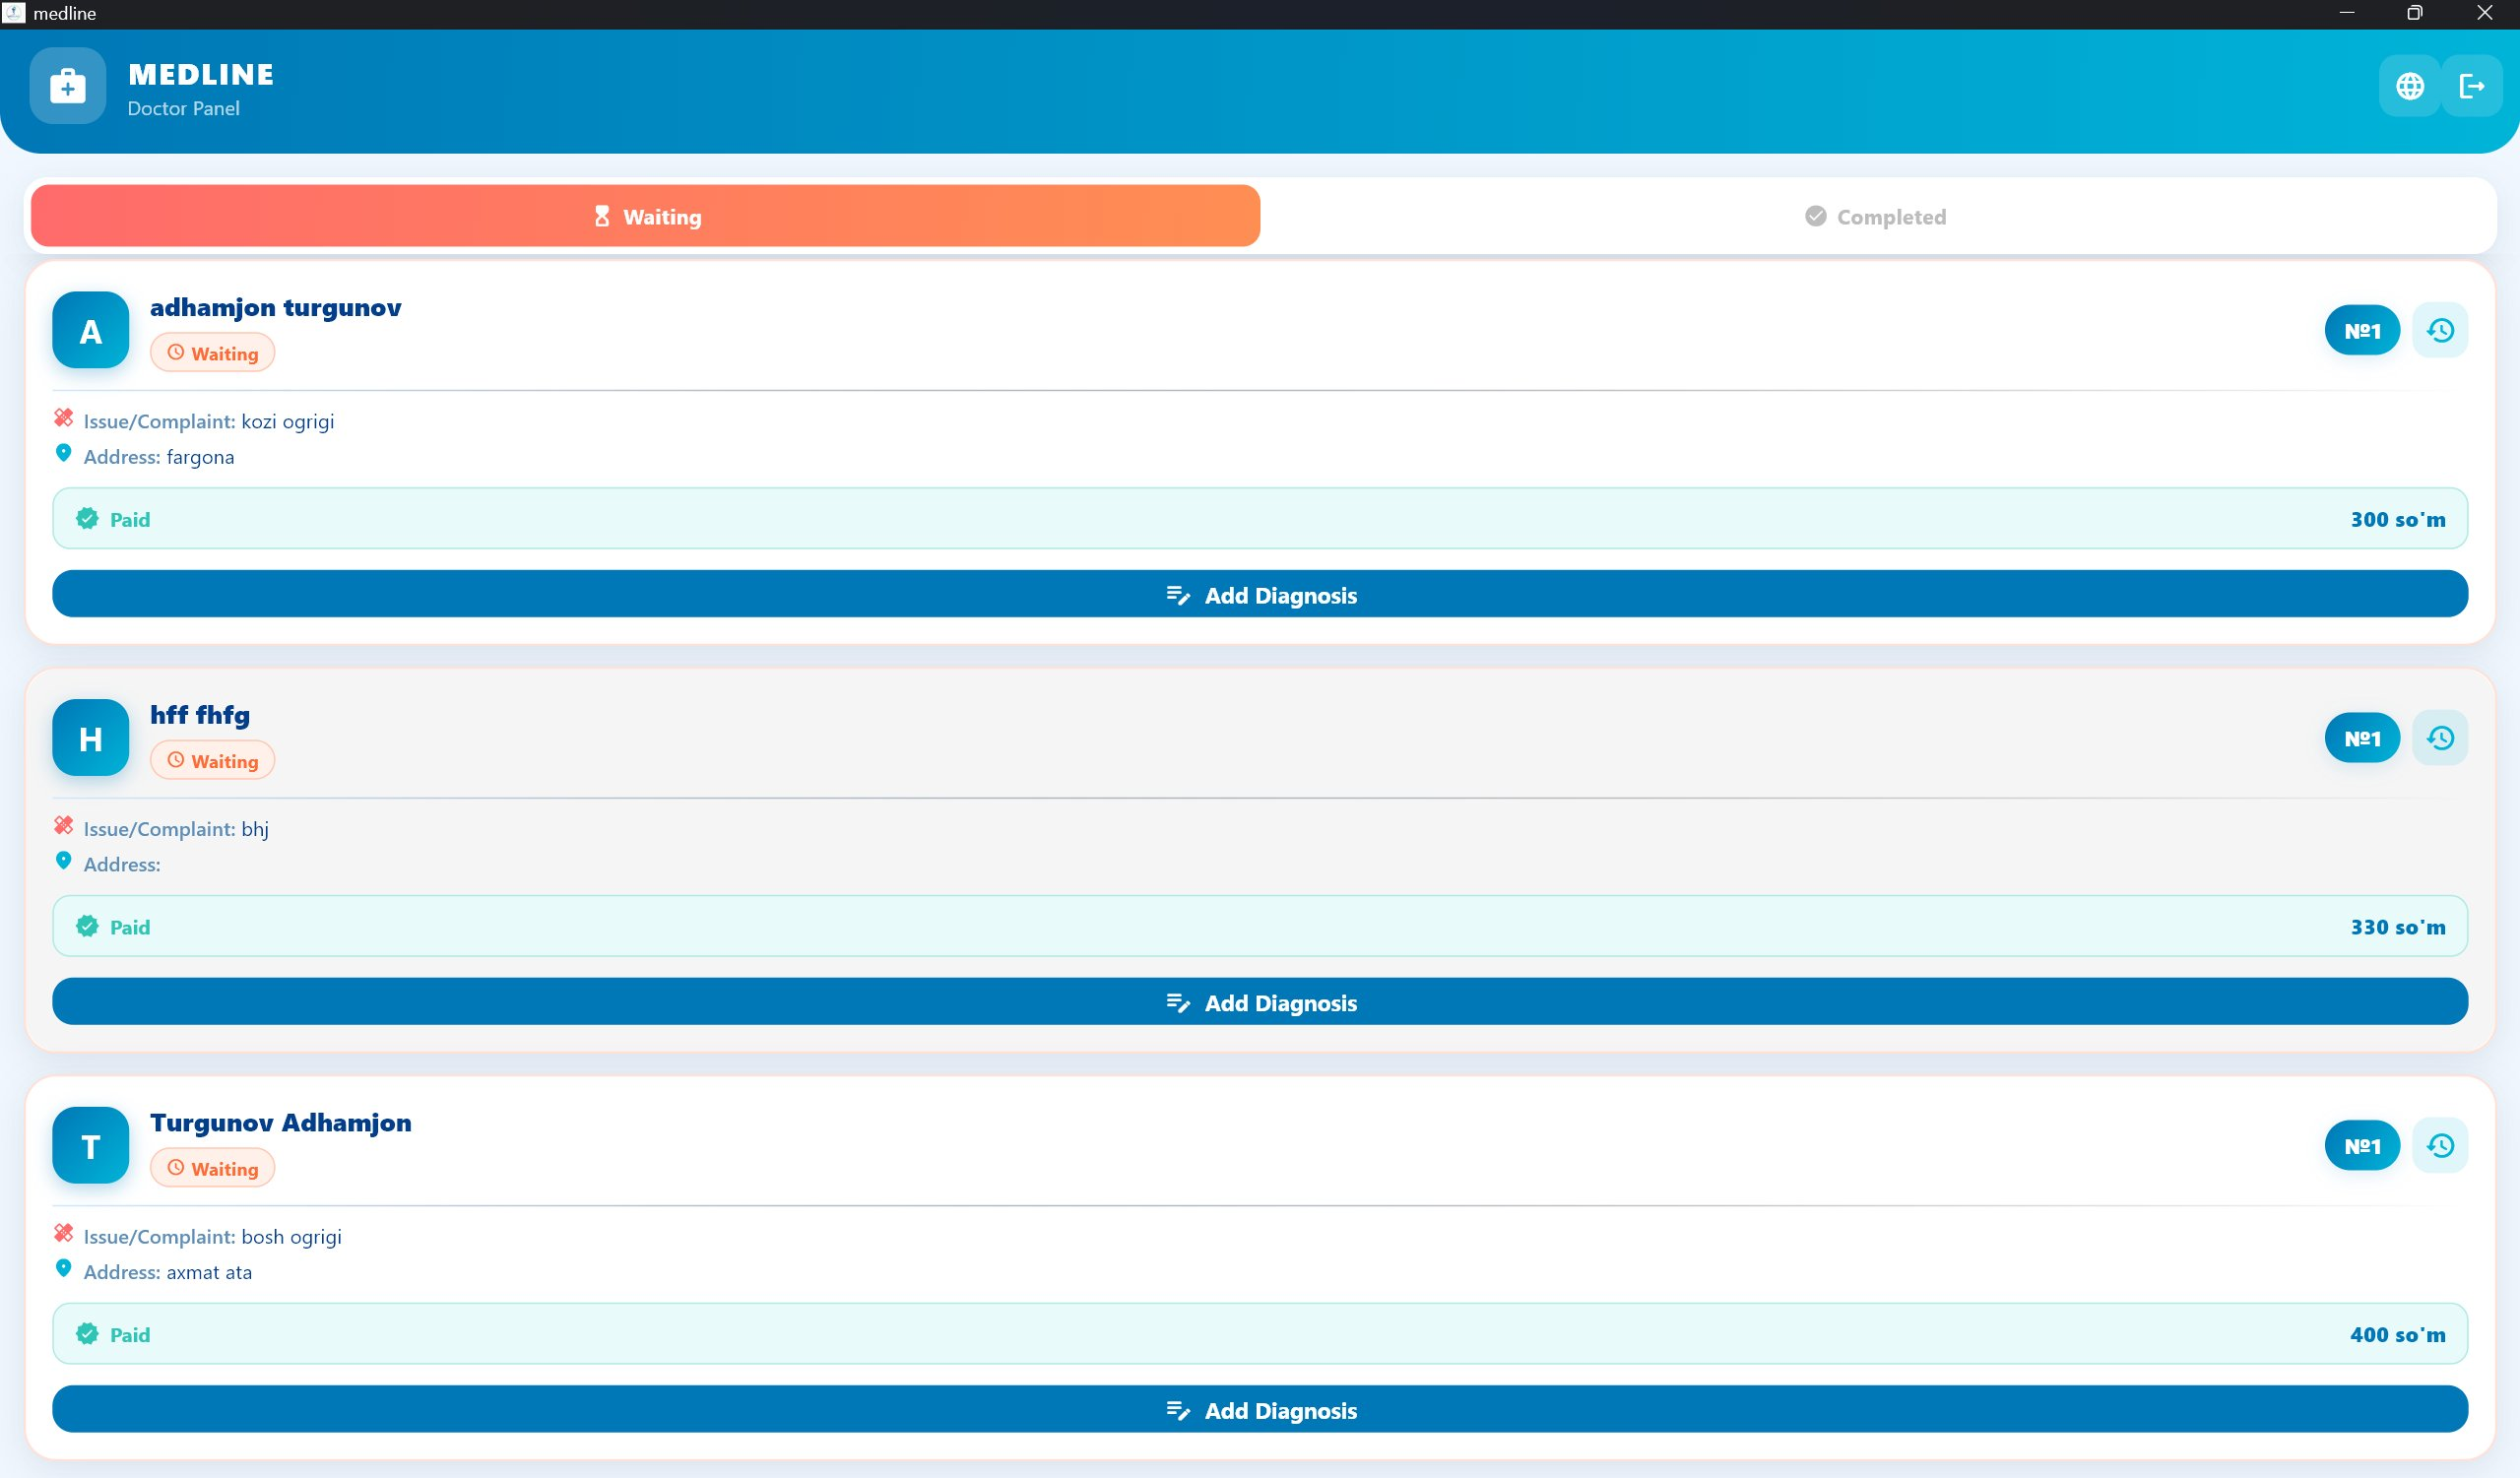
\includegraphics[width=0.45\textwidth]{fig3_6_doctor.png}
  \caption{Doctor dashboard: the daily waiting-patient queue showing each
           patient's complaint, address, payment status, and the Add Diagnosis
           action.}
  \label{fig:doctor}
  \source{author's screenshot of the implemented MEDLINE application.}
\end{figure}

\subsection{Receptionist Dashboard}

The Receptionist screen implements real-time patient search via prefix matching
on the \texttt{fullName} field and new-patient registration. The registration
form collects demographic fields with client-side validation before a Firestore
\texttt{add()} call creates the patient document. The
\texttt{AppDateUtils.formatTimestamp()} utility renders Firestore
\texttt{Timestamp} objects in a locale-aware format throughout the screen.

\begin{figure}[htbp]
  \centering
  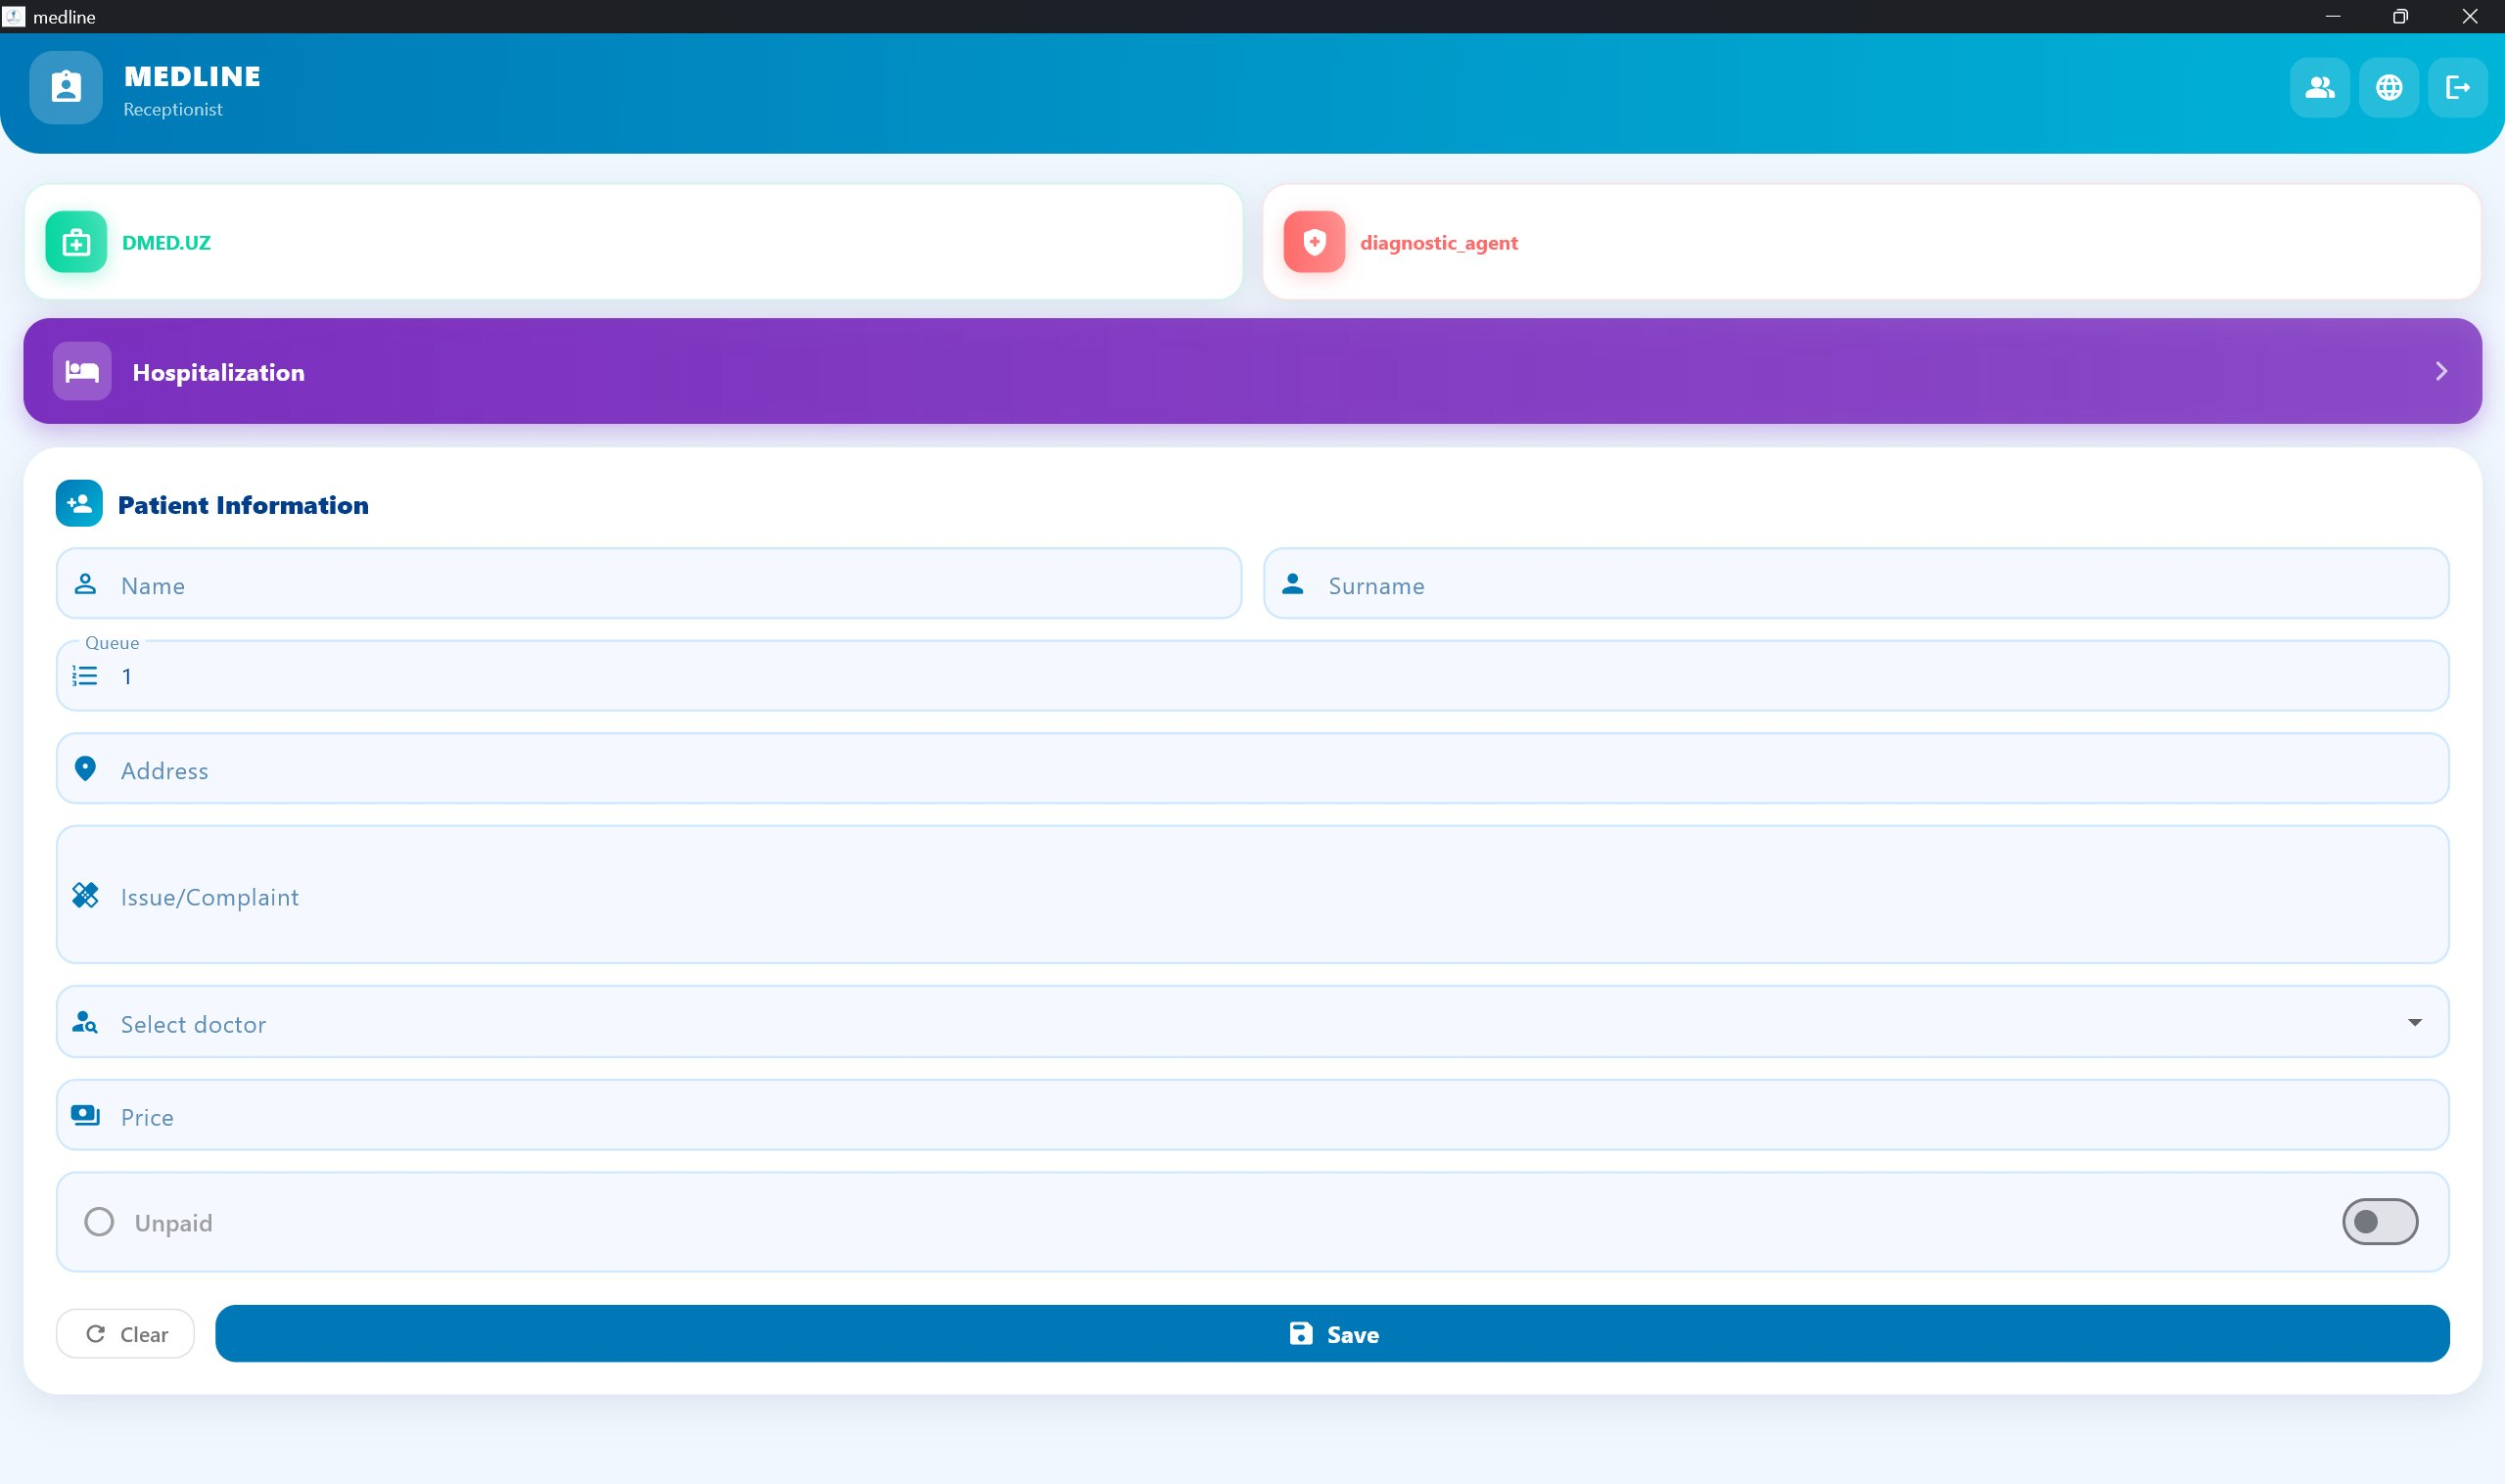
\includegraphics[width=0.45\textwidth]{fig3_7_receptionist.png}
  \caption{Receptionist dashboard: the patient-registration form with
           quick-access modules (DMED.UZ, diagnostic agent, and
           hospitalization).}
  \label{fig:receptionist}
  \source{author's screenshot of the implemented MEDLINE application.}
\end{figure}

\subsection{Laboratory Dashboard}

The Laboratory dashboard streams pending lab requests using
\texttt{where('status', isEqualTo: 'pending')}. Staff enter quantitative or
qualitative results; pressing \emph{Complete} triggers a Firestore
\texttt{update()} setting status to completed and recording \texttt{completedAt}
as a server timestamp. Completed results can be rendered as PDF using the
\texttt{pdf} package.

\subsection{Pharmacy Dashboard}

The Pharmacy dashboard mirrors the Laboratory pattern applied to
\texttt{prescriptions}: incoming prescriptions are listed, and the dispense
action updates \texttt{dispensed} to \texttt{true} and records
\texttt{dispensedAt}. Stock management flags items whose requested quantity
exceeds available stock.

\subsection{Hospitalization Dashboard}

The Hospitalization dashboard renders a grid of bed-status cards colour-coded by
occupancy. Staff admit a patient by linking a patient document to a bed
document, update daily status notes, and discharge by clearing the bed's
\texttt{patientId} field.

\begin{figure}[htbp]
  \centering
  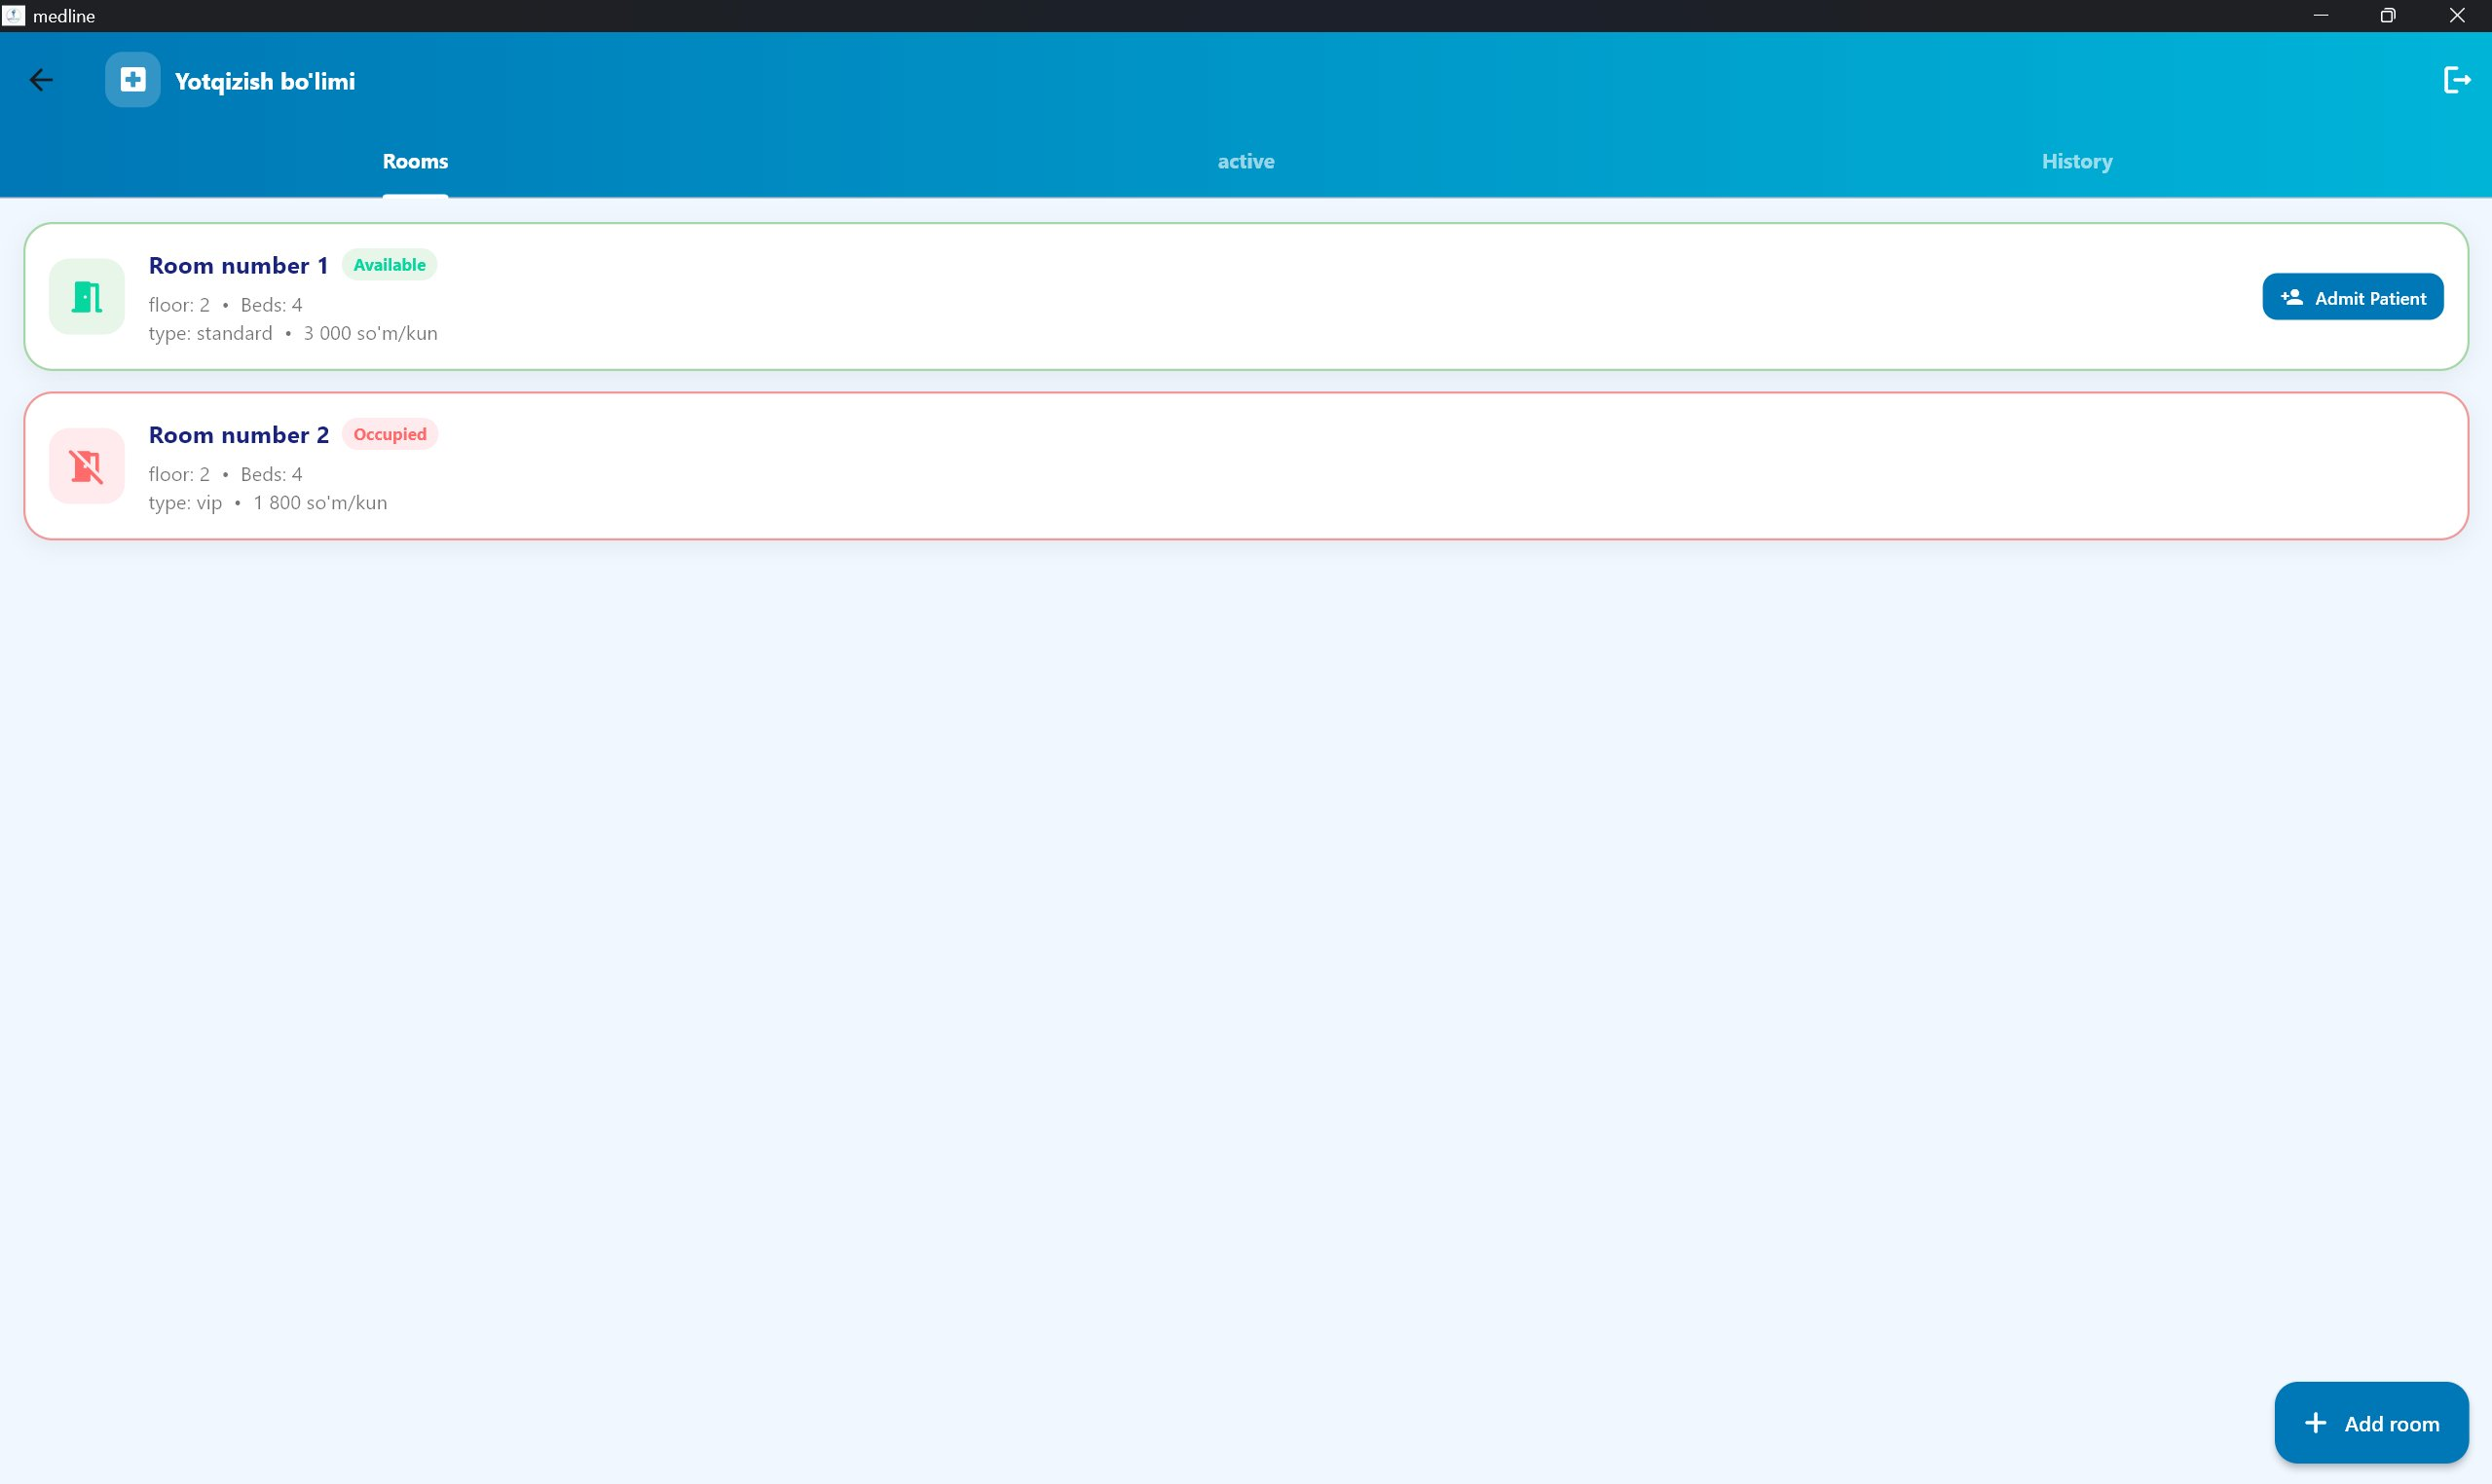
\includegraphics[width=0.45\textwidth]{fig3_8_hospitalization.png}
  \caption{Hospitalization dashboard: the ward room list showing each room's
           availability status, bed count, type, and daily price, with an Admit
           Patient action.}
  \label{fig:hospitalization}
  \source{author's screenshot of the implemented MEDLINE application.}
\end{figure}

\section{Diagnostic Decision-Support Module}
\label{sec:diagnostic}

Beyond transactional record-keeping, MEDLINE integrates a rule-based diagnostic
decision-support module that gives the system its analytical, ``intelligent''
capability. The module embeds a curated medical knowledge base and a transparent
scoring procedure to rank candidate conditions against a patient's reported
symptoms. In the taxonomy of clinical decision-support systems, this is a
\emph{knowledge-based} CDSS: its inferences are produced by explicit
human-curated rules rather than by a trained statistical model~\cite{sutton2020}.
This design choice is deliberate --- in a clinical setting, the transparency and
auditability of an explicit rule base are decisive advantages over an opaque
predictor.

\subsection{Knowledge Base}

The knowledge base (\texttt{lib/screens/diagnostic\_web\_screen.dart}) encodes
31 conditions. Each condition is represented as a document containing its name,
a recommended specialist, and a list of characteristic symptoms expressed in
Uzbek. The complete vocabulary of distinct symptoms is derived at runtime from
the union of all condition symptom lists, ensuring the selectable symptom set
and the knowledge base never drift out of sync.

\subsection{Symptom-Matching and Scoring}

When the clinician selects a set of observed symptoms, the module scores every
condition in the knowledge base using two complementary measures, computed in
the \texttt{\_getResults()} method shown in Listing~\ref{lst:scoring} and
formalised in Algorithm~\ref{alg:scoring}. For a candidate condition with
symptom set $D$ and a selected-symptom set $S$, let $M = D \cap S$ be the
matched symptoms. The module computes
\begin{equation}
  \mathrm{match}(D) = \frac{|M|}{|S|}\times 100\%,
  \qquad
  \mathrm{coverage}(D) = \frac{|M|}{|D|}\times 100\%.
  \label{eq:scoring}
\end{equation}
The match score (precision-like) expresses how many of the clinician's selected
symptoms are explained by the condition, while coverage (recall-like) expresses
how completely the condition's own symptom profile is satisfied. Conditions are
ranked by match score in descending order; an optional high-risk filter retains
only conditions with a match score of at least 60\%, and each result is
colour-coded by risk band (red $\geq 80\%$, orange $\geq 60\%$,
amber $\geq 40\%$).

\begin{algorithm}[htbp]
  \caption{Symptom-matching and condition scoring}
  \label{alg:scoring}
  \begin{algorithmic}[1]
    \Require selected-symptom set $S$, knowledge base $K$
    \If{$S = \emptyset$}
      \State \Return $\emptyset$
    \EndIf
    \State $R \gets \emptyset$
    \ForAll{condition $D \in K$}
      \State $M \gets \{\, s \in D.\text{symptoms} : s \in S \,\}$
      \If{$|M| > 0$}
        \State $D.\text{match} \gets \mathrm{round}(|M|/|S| \times 100)$
        \State $D.\text{coverage} \gets \mathrm{round}(|M|/|D.\text{symptoms}| \times 100)$
        \State $R \gets R \cup \{D\}$
      \EndIf
    \EndFor
    \If{high-risk filter enabled}
      \State $R \gets \{\, D \in R : D.\text{match} \geq 60 \,\}$
    \EndIf
    \State sort $R$ by $D.\text{match}$ descending
    \State \Return $R$
  \end{algorithmic}
\end{algorithm}

\begin{lstlisting}[caption={Condition-scoring logic in \texttt{\_getResults()}.},label={lst:scoring}]
List<Map<String, dynamic>> _getResults() {
  if (selectedSymptoms.isEmpty) return [];
  var results = diseases.map((d) {
    final matched = (d['symptoms'] as List<String>)
        .where((s) => selectedSymptoms.contains(s))
        .toList();
    final percentage = matched.isNotEmpty
        ? (matched.length / selectedSymptoms.length * 100).round()
        : 0;
    final coverage = matched.isNotEmpty
        ? (matched.length / (d['symptoms'] as List).length * 100).round()
        : 0;
    return {...d, 'matched': matched,
            'percentage': percentage, 'coverage': coverage};
  }).where((r) => r['percentage'] > 0).toList();

  if (_showOnlyHighRisk) {
    results = results.where((r) => r['percentage'] >= 60).toList();
  }
  switch (_sortBy) {
    case 'percentage':
      results.sort((a, b) => b['percentage'].compareTo(a['percentage']));
      break;
    case 'name':
      results.sort((a, b) => a['name'].compareTo(b['name']));
      break;
  }
  return results;
}
\end{lstlisting}

The end-to-end flow of the module --- from symptom selection through scoring,
filtering, and ranked presentation --- is summarised in
Figure~\ref{fig:pipeline}.

\begin{figure}[htbp]
  \centering
  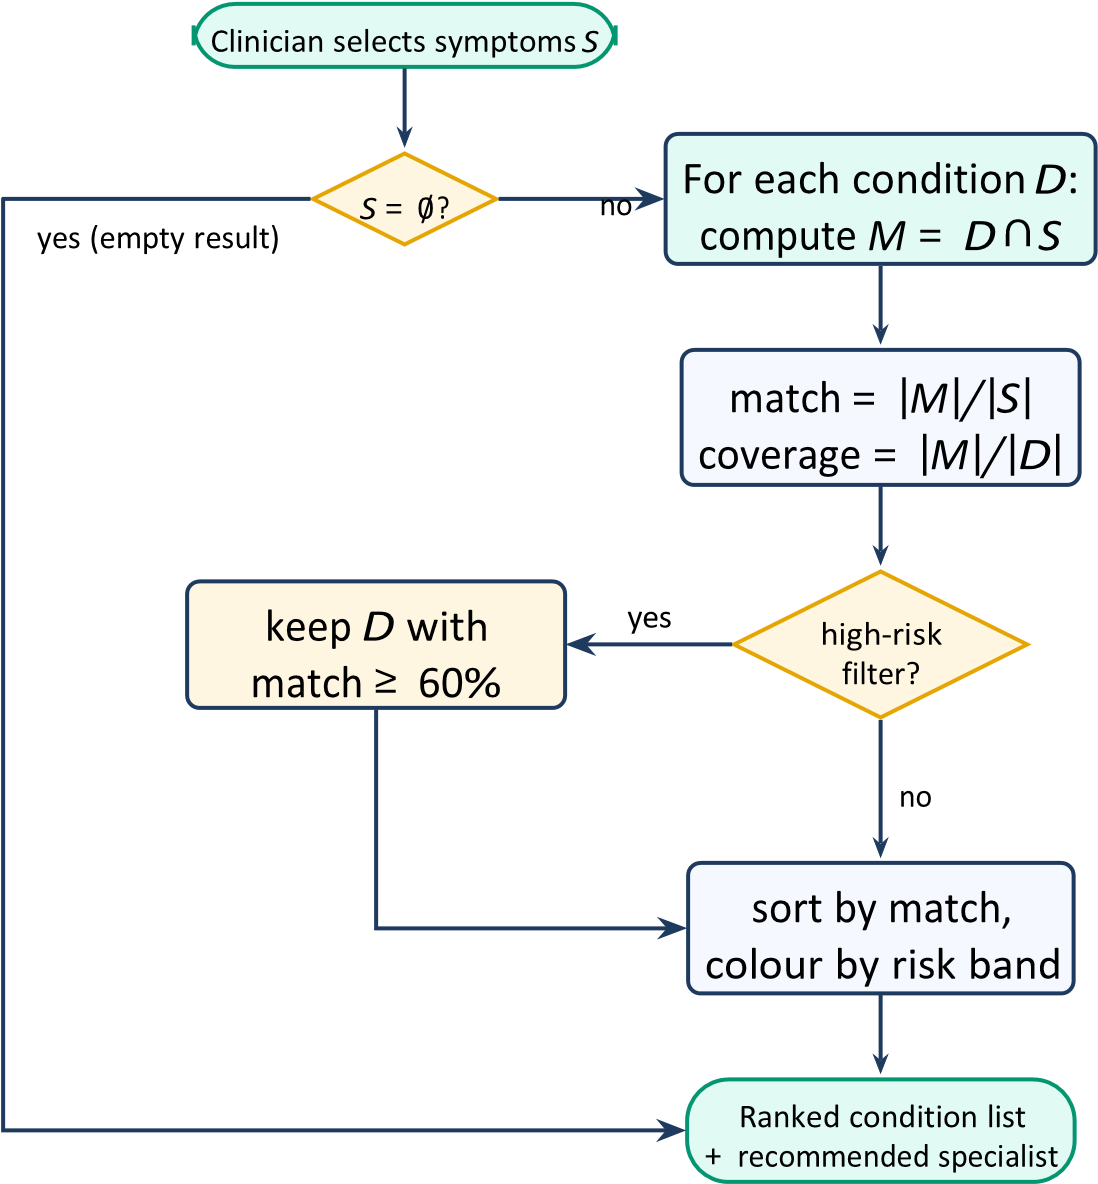
\includegraphics[width=0.85\textwidth]{fig3_3_diagnostic_pipeline.png}
  \caption{Diagnostic decision-support pipeline: from symptom selection to
           ranked output.}
  \label{fig:pipeline}
  \source{author, derived from \texttt{diagnostic\_web\_screen.dart}.}
\end{figure}

It must be emphasised that this module is a decision \emph{aid}, not an
autonomous diagnostician: it surfaces and ranks possibilities for a qualified
clinician to consider, and every result is accompanied by the matched symptoms
and a recommended specialist so that the reasoning behind each suggestion
remains fully inspectable.

\section{Multilingual Support}

The \texttt{LanguageProvider} holds a compile-time translation map of more than
200 string keys across four locales: Uzbek (UZB), English (ENG), Russian (RUS),
and Kyrgyz (KYR). The active language is persisted via
\texttt{SharedPreferences}. All UI strings are accessed through
\texttt{lang.translate(key)}, enabling runtime language switching without an
application restart. This design keeps localisation logic entirely within the
Provider layer, decoupled from widget code; the lookup itself, with its safe key
fallback, is shown in Listing~\ref{lst:translate} of Appendix~\ref{app:code}.

\section{Theme System}

\texttt{ThemeProvider} defines two colour palettes: a dark palette
(navy \texttt{\#0A2D4A}, teal \texttt{\#4DB6AC}) and a light palette (white
background, green \texttt{\#00897B}). Derived properties
(\texttt{cardBackground}, \texttt{inputFill}, \texttt{textPrimary}) abstract
palette details away from screen widgets, and a \texttt{glassDecoration()}
factory produces the frosted-glass card style used uniformly across all six
dashboards. The theme mode is persisted via \texttt{SharedPreferences} and
restored on startup.

\section{Automated PDF Report Generation}

PDF reports are generated client-side using the \texttt{pdf} and
\texttt{printing} packages~\cite{pdfpkg2024}. The generation process has four
steps: (1)~create a \texttt{pw.Document} instance; (2)~fetch the required data
from Firestore; (3)~build a \texttt{pw.Page} with a clinic header, generation
timestamp, and a structured data table; and (4)~call
\texttt{Printing.layoutPdf()} to render and share the document. The
\texttt{path\_provider} package resolves the platform-appropriate temporary
directory, and \texttt{open\_filex} launches the PDF in the device's native
viewer. Because no server endpoint is involved, patient data remains on-device
throughout rendering --- a privacy property revisited in Chapter~4.

\section{Sub-Conclusions}

MEDLINE's architecture distributes responsibilities cleanly across five layers.
Six role-specific dashboards implement every stakeholder use case identified in
Chapter~2. The Provider-based multilingual system supports four locales without
code duplication, and the rule-based diagnostic module adds transparent decision
support on top of the transactional core. The serverless Firebase backend
eliminates infrastructure management, and client-side PDF generation preserves
patient-data privacy during report rendering. Chapter~4 evaluates whether this
design satisfies all requirements stated in Chapter~2.

%============================== CHAPTER 4 =====================================
\chapter{System Evaluation, Discussion, and Future Work}

This chapter evaluates the implemented MEDLINE system against the functional and
non-functional requirements defined in Chapter~2, discusses the principal
architectural trade-offs, assesses the research hypothesis, states the
limitations of the study honestly, and proposes concrete directions for future
development.

\section{Functional Requirement Evaluation}

All ten functional requirements were evaluated through end-to-end manual testing
on Android (API~33), Chrome Web, and Windows desktop builds of MEDLINE.
Table~\ref{tab:freval} presents the results.

\begin{table}[htbp]
  \centering
  \caption{Functional requirement evaluation results.}
  \label{tab:freval}
  \begin{tabularx}{\textwidth}{l X c}
    \toprule
    \textbf{ID} & \textbf{Requirement (abbreviated)} & \textbf{Result}\\
    \midrule
    FR-01 & Role-based authentication and routing & Pass\\
    FR-02 & Patient registration with validation & Pass\\
    FR-03 & Real-time patient queue for doctors & Pass\\
    FR-04 & Consultation notes and ICD-10 entry & Pass\\
    FR-05 & Laboratory request and result workflow & Pass\\
    FR-06 & Prescription and dispensing workflow & Pass\\
    FR-07 & Hospitalization bed management & Pass\\
    FR-08 & Payment recording and revenue stats & Pass\\
    FR-09 & Client-side PDF report generation & Pass\\
    FR-10 & Runtime multilingual UI switching & Pass\\
    \bottomrule
  \end{tabularx}
  \source{author, end-to-end manual testing.}
\end{table}

All ten functional requirements passed verification. The real-time patient queue
(FR-03) reflected registration events within one to two seconds on a local Wi-Fi
connection, comfortably satisfying NFR-01 (the three-second target).

\section{Non-Functional Requirement Evaluation}

\subsection{Performance (NFR-01)}

Dashboard load times were measured using Flutter DevTools on a mid-range Android
device (Snapdragon 695, 6\,GB RAM) over a 50\,Mbps LTE connection. The Admin
dashboard --- which performs the largest Firestore query, retrieving all payment
documents --- loaded in approximately 1.8 seconds from a cold start. The Doctor
and Receptionist dashboards, with narrower date-range queries, loaded in under
one second. Figure~\ref{fig:loadtimes} plots the measured load times against the
three-second NFR-01 target; every dashboard falls well within budget, so NFR-01
is satisfied.

\begin{figure}[htbp]
  \centering
  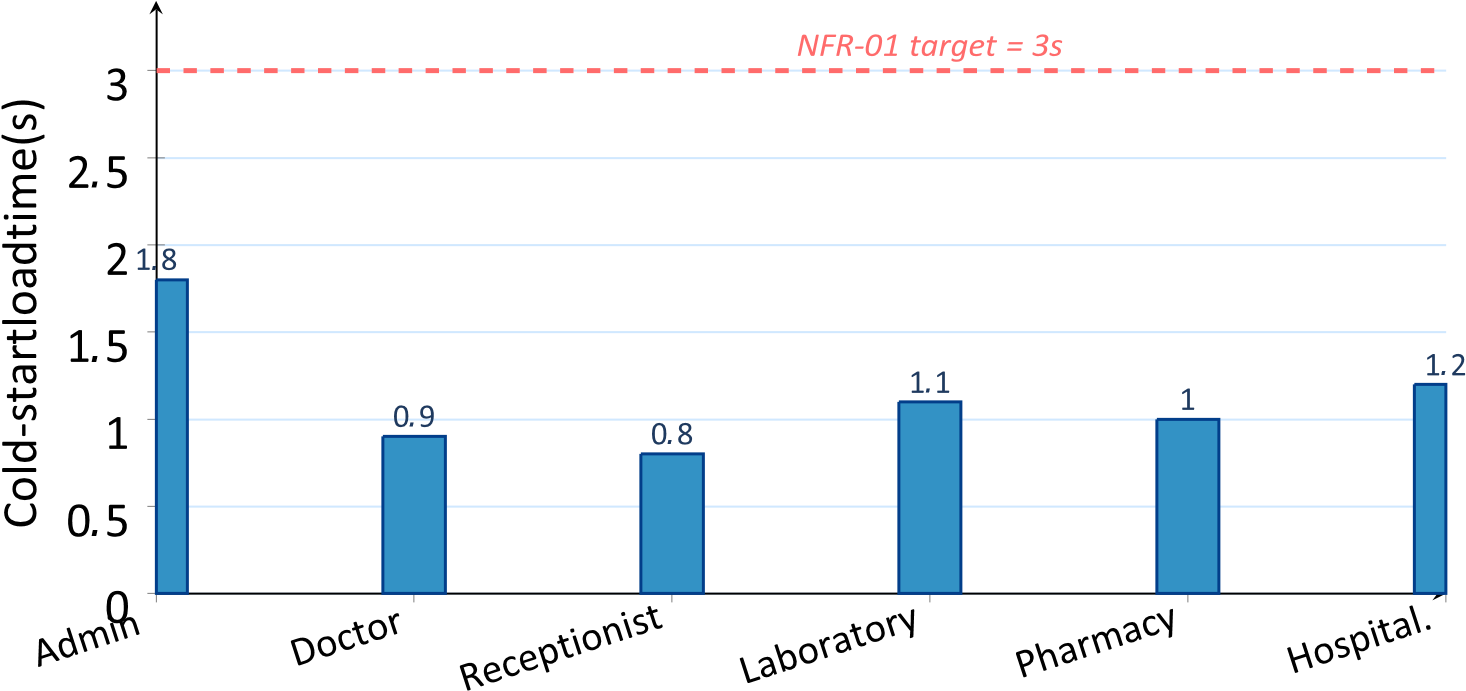
\includegraphics[width=0.85\textwidth]{fig4_1_load_times.png}
  \caption{Measured dashboard cold-start load times against the 3-second NFR-01
           target.}
  \label{fig:loadtimes}
  \source{author, measured with Flutter DevTools (Snapdragon 695,
          50\,Mbps LTE).}
\end{figure}

\subsection{Security (NFR-03)}

Firebase Authentication enforces TLS for all credential exchange. Firestore
Security Rules restrict document reads and writes based on the authenticated UID
and role field, satisfying NFR-03 at both the transport and storage
layers~\cite{fernandez2013}. At the application layer, \texttt{AuthWrapper}
routing ensures that a user with role \texttt{pharmacy} cannot navigate to the
\texttt{AdminDashboard}, because that route is never added to the navigation
stack for non-admin roles.

\subsection{Portability (NFR-05)}

The codebase was compiled and executed on Android (API~33), Chrome (Web), and
Windows desktop without platform-specific code modifications beyond the
\texttt{firebase\_options.dart} configuration file. NFR-05 is satisfied.

\subsection{Usability (NFR-04)}

The application sets \texttt{useMaterial3: true} in its \texttt{ThemeData} and
follows Material Design 3 component guidelines~\cite{material2024}. The
four-language UI supports clinical staff who may not be proficient in English.
Loading indicators, form validation before submission, and labelled icon buttons
address Nielsen and Budiu's mobile usability heuristics of system-status
visibility, error prevention, and recognition over recall~\cite{nielsen2020}.

\section{Discussion of Architectural Trade-offs}

The serverless Firebase backend eliminates infrastructure management but
introduces vendor lock-in: migrating to a self-hosted NoSQL database would
require rewriting all Firestore query and listener logic. For the target
audience --- small private clinics with no dedicated IT staff --- operational
simplicity outweighs portability concerns. This trade-off is consistent with the
project constraints identified in Chapter~2.

Client-side PDF generation keeps patient data on-device during rendering, which
is a privacy advantage. However, it places computational load on the client and
may produce slower exports on low-end devices for large data sets. A future
hybrid approach --- server-side rendering for batch reports, client-side for
single-patient documents --- could address this.

The \texttt{CacheManager} class in the current implementation is an in-memory
dictionary with no eviction policy or persistence; it does not survive
application restarts. Firestore's built-in offline persistence partially
compensates, but a structured caching layer using Hive or SQLite would improve
offline robustness for clinics with intermittent connectivity.

\section{Hypothesis Validation}

The research hypothesis stated that a cross-platform Flutter/Firebase application
can fulfil the core registration, monitoring, and reporting requirements of a
multi-department clinic within a single shared codebase. All ten functional
requirements were verified as satisfied on three distinct platforms from one
codebase (Table~\ref{tab:freval}). The hypothesis is therefore confirmed.

\section{Limitations of the Study}

\paragraph{Testing scope.} Evaluation was conducted through manual functional
testing only. No automated unit, widget, or integration tests were implemented
within the scope of this thesis.

\paragraph{Scale.} The system was tested with synthetic data sets of up to 200
patient records. Firestore behaviour under tens of thousands of documents with
complex composite queries was not benchmarked.

\paragraph{Clinical validation.} MEDLINE was not deployed in a live clinical
environment, and no usability evaluation was conducted with actual clinical
staff.

\paragraph{ICD-10 integration.} Diagnosis codes are entered as free-text
strings; no ICD-10 lookup or validation service is integrated, risking
inconsistent coding.

\section{Future Work}
\label{sec:futurework}

\paragraph{Automated testing.} Implement widget and integration tests using
\texttt{flutter\_test} to establish a regression safety net before clinical
deployment.

\paragraph{Security-rule hardening.} Write and validate explicit
collection-level Firestore rules using the Firebase Emulator Suite to replace
permissive development rules.

\paragraph{ICD-10 autocomplete.} Integrate a local ICD-10 code database to
provide type-ahead search during doctor consultation, reducing input errors.

\paragraph{Push notifications.} Use Firebase Cloud Messaging to alert doctors
when laboratory results are ready and pharmacists when new prescriptions arrive.

\paragraph{Analytics.} Export aggregated Firestore data to BigQuery to support
longitudinal reporting and trend analysis for clinic managers.

\paragraph{Clinical pilot.} Partner with a small private clinic for a structured
deployment, collect usability feedback using the System Usability Scale, and
iterate.

\section{Sub-Conclusions}

All ten functional requirements were verified as satisfied. The performance,
security, and portability non-functional requirements were met within the scope
of testing. The research hypothesis was confirmed. Architectural trade-offs
inherent in the serverless Firebase model and in client-side PDF generation were
analysed. The primary limitations are the absence of automated testing and live
clinical validation. Six concrete future-development directions were proposed,
with automated testing, security-rule hardening, and a clinical pilot as the
highest-priority next steps.

%============================== CONCLUSIONS ===================================
\chapter*{Conclusions}
\addcontentsline{toc}{chapter}{Conclusions}

This Bachelor's thesis designed and implemented MEDLINE, an integrated,
role-based clinic-management system built on Flutter and Firebase, and evaluated
the result against a defined set of functional and non-functional requirements.
The following conclusions confirm the achievement of all four study tasks.

Task~1 (Chapter~1) was completed by surveying healthcare information-system
theory, cross-platform mobile frameworks, role-based access control, Firestore
document architecture, the Provider pattern, clinical decision support, and PDF
generation. Technology choices were explicitly justified: Flutter was selected
for its cross-platform compiled rendering performance, Firebase for its
serverless, real-time, zero-infrastructure model, and Provider for its
low-boilerplate state management adequate to the project's scope.

Task~2 (Chapter~2) was completed by identifying six stakeholder groups,
cataloguing operational pain points, eliciting ten functional and six
non-functional requirements, and comparing MEDLINE with existing systems. The
comparison confirmed that no readily available solution combines all of a
serverless backend, real-time multi-role dashboards, automated PDF reporting,
and cross-platform deployment at zero licensing cost.

Task~3 (Chapter~3) was completed by implementing MEDLINE across a five-layer
architecture. Six role-specific dashboards (Admin, Doctor, Receptionist,
Pharmacy, Laboratory, and Hospitalization) were built, together with a
rule-based diagnostic decision-support module, a four-language UI system, a
dual-theme engine, and a client-side PDF generation module --- all delivered
from a single Flutter codebase deployable on Android, iOS, and the Web.

Task~4 (Chapter~4) was completed by verifying all ten functional requirements
through end-to-end testing on three platforms. Dashboard load times were
measured below the three-second target, and the security and portability
requirements were confirmed. Architectural trade-offs, limitations, and six
future development directions were analysed.

The research hypothesis --- that a Flutter/Firebase cross-platform application
can fulfil the core registration, monitoring, and reporting requirements of a
multi-department clinic within a single shared codebase --- was confirmed.

Therefore, the aim of the thesis has been achieved. MEDLINE provides a
functional, portable, and maintainable clinic-management platform that addresses
the documented operational deficiencies of small private healthcare facilities.
The work's practical value lies in demonstrating a zero-infrastructure
architecture that places a complete multi-department clinical workflow ---
including transparent diagnostic decision support --- within reach of clinics
that lack dedicated IT resources. Future work should prioritise automated
testing, Firestore security-rule hardening, ICD-10 integration, and a structured
clinical pilot to validate usability with real end-users.

%============================== REFERENCES ====================================
\begin{thebibliography}{99}
\addcontentsline{toc}{chapter}{References}

\bibitem{who2019} World Health Organization, ``WHO Guideline: Recommendations on
  Digital Interventions for Health System Strengthening,'' \emph{WHO Technical
  Report Series}, 2019.

\bibitem{wager2017} K. A. Wager, F. W. Lee, and J. P. Glaser, \emph{Health Care
  Information Systems: A Practical Approach for Health Care Management}, 4th ed.
  San Francisco: Jossey-Bass, 2017.

\bibitem{kruse2018} C. S. Kruse, A. Stein, H. Thomas, and H. Kaur, ``The Use of
  Electronic Health Records to Support Population Health,'' \emph{Journal of
  Medical Systems}, vol.~42, no.~11, p.~214, 2018.

\bibitem{mesko2020} B. Mesk\'o et al., ``Digital Health is a Cultural
  Transformation of Traditional Healthcare,'' \emph{mHealth}, vol.~3, p.~38,
  2020.

\bibitem{nawrocki2021} P. Nawrocki et al., ``A Comparison of Native and
  Cross-Platform Frameworks for Mobile Applications,'' \emph{Computer}, vol.~54,
  no.~3, pp.~18--27, 2021.

\bibitem{pinto2020} C. M. Pinto and C. Coutinho, ``From Native to Cross-platform
  Hybrid Development,'' in \emph{Proc. ICTE}, 2020, pp.~1--4.

\bibitem{biorn2020} A. Biorn-Hansen, T. A. Majchrzak, and T.-M. Gr\o nli,
  ``Progressive Web Apps: The Possible Web-native Unifier for Mobile
  Development,'' in \emph{Proc. WEBIST}, 2020, pp.~344--351.

\bibitem{majchrzak2018} T. A. Majchrzak, A. Biorn-Hansen, and T.-M. Gr\o nli,
  ``Progressive Web Apps: the Definite Approach to Cross-Platform
  Development?'' in \emph{Proc. HICSS}, 2018, pp.~5735--5744.

\bibitem{flutter2024} Google, ``Flutter --- Build Apps for Any Screen,'' 2024.
  [Online]. Available: \url{https://flutter.dev/}

\bibitem{flutterarch2024} Google, ``Flutter Architectural Overview,'' 2024.
  [Online]. Available:
  \url{https://docs.flutter.dev/resources/architectural-overview}

\bibitem{windmill2020} E. Windmill, \emph{Flutter in Action}. Shelter Island,
  NY: Manning Publications, 2020.

\bibitem{dart2024} Google, ``Dart Programming Language,'' 2024. [Online].
  Available: \url{https://dart.dev/}

\bibitem{sandhu1996} R. S. Sandhu, E. J. Coyne, H. L. Feinstein, and
  C. E. Youman, ``Role-Based Access Control Models,'' \emph{Computer}, vol.~29,
  no.~2, pp.~38--47, 1996.

\bibitem{fernandez2013} J. L. Fern\'andez-Alem\'an et al., ``Security in
  Electronic Health Records: A Systematic Review,'' \emph{Journal of Biomedical
  Informatics}, vol.~46, no.~3, pp.~541--562, 2013.

\bibitem{sadalage2013} P. J. Sadalage and M. Fowler, \emph{NoSQL Distilled}.
  Upper Saddle River, NJ: Addison-Wesley, 2013.

\bibitem{firestore2024} Google Firebase, ``Cloud Firestore Documentation,''
  2024. [Online]. Available: \url{https://firebase.google.com/docs/firestore}

\bibitem{provider2024} pub.dev, ``Provider --- A Wrapper Around
  InheritedWidget,'' 2024. [Online]. Available:
  \url{https://pub.dev/packages/provider}

\bibitem{pdfpkg2024} pub.dev, ``pdf --- A PDF Producer for Dart,'' 2024.
  [Online]. Available: \url{https://pub.dev/packages/pdf}

\bibitem{adebayo2021} K. J. Adebayo and M. E. H. Lim, ``Mobile-based Patient
  Management System for Developing Countries,'' \emph{International Journal of
  Computer Applications}, vol.~174, no.~8, pp.~21--28, 2021.

\bibitem{firebaseauth2024} Google Firebase, ``Firebase Authentication,'' 2024.
  [Online]. Available: \url{https://firebase.google.com/docs/auth}

\bibitem{firebase2024} Google Firebase, ``Firebase --- App Development
  Platform,'' 2024. [Online]. Available: \url{https://firebase.google.com/}

\bibitem{payne2019} R. Payne, \emph{Beginning App Development with Flutter}.
  Dallas, TX: Apress, 2019.

\bibitem{nielsen2020} J. Nielsen and R. Budiu, \emph{Mobile Usability}.
  Berkeley, CA: New Riders, 2020.

\bibitem{material2024} Google, ``Material Design 3,'' 2024. [Online]. Available:
  \url{https://m3.material.io/}

\bibitem{sommerville2016} I. Sommerville, \emph{Software Engineering}, 10th ed.
  Boston: Pearson, 2016.

\bibitem{sutton2020} R. T. Sutton et al., ``An Overview of Clinical Decision
  Support Systems: Benefits, Risks, and Strategies for Success,'' \emph{npj
  Digital Medicine}, vol.~3, no.~17, 2020.

\end{thebibliography}

%============================== APPENDIX A ====================================
\appendix
\chapter{Key Source Code Listings}
\label{app:code}

This appendix reproduces representative excerpts of the MEDLINE source code that
illustrate the design decisions discussed in Chapter~3.

\section{AuthWrapper --- Role-Based Routing}

The \texttt{\_buildDashboard()} method implements the role-routing logic at the
application's authentication boundary, mapping each stored role to its dashboard
widget and falling back safely for an unrecognised role.

\begin{lstlisting}[caption={\texttt{\_buildDashboard()} role-to-widget dispatch
  in \texttt{auth\_wrapper.dart}.},label={lst:builddashboard}]
Widget _buildDashboard(String role) {
  switch (role) {
    case 'admin':           return const AdminDashboard();
    case 'doctor':          return const DoctorDashboard();
    case 'receptionist':    return const ReceptionistDashboard();
    case 'pharmacy':        return const PharmacyDashboard();
    case 'laboratory':      return const LaboratoryDashboard();
    case 'hospitalization': return const HospitalizationDashboard();
    default:
      return Scaffold(
        body: Center(child: Text('Unknown role: $role')),
      );
  }
}
\end{lstlisting}

\section{LanguageProvider --- Runtime Translation}

The \texttt{translate()} method performs a two-level map lookup, returning the
key itself as a safe fallback if a translation is missing;
\texttt{setLanguage()} persists the active locale and notifies listeners so the
UI rebuilds without a restart.

\begin{lstlisting}[caption={Runtime translation and locale persistence in
  \texttt{language\_provider.dart}.},label={lst:translate}]
String translate(String key) {
  return _translations[key]?[_currentLanguage] ?? key;
}

Future<void> setLanguage(String lang) async {
  _currentLanguage = lang;
  final prefs = await SharedPreferences.getInstance();
  await prefs.setString('language', lang);
  notifyListeners();
}
\end{lstlisting}

\section{AppDateUtils --- Locale-Aware Timestamp Formatting}

The \texttt{formatTimestamp()} utility renders Firestore \texttt{Timestamp}
objects with smart today/yesterday labels and locale-appropriate date patterns.

\begin{lstlisting}[caption={Locale-aware timestamp formatting in
  \texttt{date\_utils.dart}.},label={lst:dateutils}]
static String formatTimestamp(Timestamp? timestamp, BuildContext context,
    {bool includeTime = true}) {
  if (timestamp == null) return lang.translate('not_specified');
  final date = timestamp.toDate();
  final dateOnly = DateTime(date.year, date.month, date.day);
  if (dateOnly == today) {
    return '${lang.translate("today")} '
           '${DateFormat("HH:mm").format(date)}';
  }
  final pattern = lang.currentLanguage == 'ENG'
      ? 'MMMM dd, yyyy, hh:mm a'
      : 'dd MMMM yyyy, HH:mm';
  return DateFormat(pattern).format(date);
}
\end{lstlisting}

%============================== APPENDIX B ====================================
\chapter{Firestore Data Schema}

This appendix details the document schema of the three most central Firestore
collections. Field types follow Firestore's native type system; the
\texttt{Timestamp} type stores a server-resolved date-time value.

\begin{table}[htbp]
  \centering
  \caption{\texttt{users} collection schema.}
  \label{tab:users}
  \begin{tabularx}{\textwidth}{l l X}
    \toprule
    \textbf{Field} & \textbf{Type} & \textbf{Description}\\
    \midrule
    \texttt{uid} & String & Firebase Auth UID (document key)\\
    \texttt{email} & String & Login email address\\
    \texttt{fullName} & String & Staff member's full name\\
    \texttt{role} & String & One of the six role identifiers\\
    \texttt{createdAt} & Timestamp & Account creation time\\
    \bottomrule
  \end{tabularx}
  \source{author.}
\end{table}

\begin{table}[htbp]
  \centering
  \caption{\texttt{patients} collection schema.}
  \label{tab:patients}
  \begin{tabularx}{\textwidth}{l l X}
    \toprule
    \textbf{Field} & \textbf{Type} & \textbf{Description}\\
    \midrule
    \texttt{fullName} & String & Patient's full name (search key)\\
    \texttt{phone} & String & Contact phone number\\
    \texttt{gender} & String & Patient gender\\
    \texttt{birthDate} & Timestamp & Date of birth\\
    \texttt{purpose} & String & Reason for visit\\
    \texttt{registeredAt} & Timestamp & Registration time\\
    \bottomrule
  \end{tabularx}
  \source{author.}
\end{table}

\begin{table}[htbp]
  \centering
  \caption{\texttt{lab\_requests} collection schema.}
  \label{tab:labrequests}
  \begin{tabularx}{\textwidth}{l l X}
    \toprule
    \textbf{Field} & \textbf{Type} & \textbf{Description}\\
    \midrule
    \texttt{patientId} & String & Reference to \texttt{patients} document\\
    \texttt{testType} & String & Requested test category\\
    \texttt{status} & String & \texttt{pending} or \texttt{completed}\\
    \texttt{result} & String & Entered test result\\
    \texttt{requestedAt} & Timestamp & Order creation time\\
    \texttt{completedAt} & Timestamp & Result completion time\\
    \bottomrule
  \end{tabularx}
  \source{author.}
\end{table}

%============================== AFFIRMATION ===================================
\chapter*{Affirmation}
\addcontentsline{toc}{chapter}{Affirmation}

Hereby I, Turgunov Adhamjon, affirm that the Bachelor's thesis was performed
independently, without the assistance of others; sources of data and definitions
taken from external sources are indicated in the thesis. This work has not been
submitted to any other examination commission and has not been published
elsewhere.

\vspace{1.5cm}
Riga, 2026

\vspace{2cm}
\noindent
\begin{tabular}{p{6cm}p{6cm}}
\hrulefill & \hrulefill\\
\centering signature & \centering Turgunov Adhamjon\\
\end{tabular}

%============================== ACKNOWLEDGMENTS ===============================
\chapter*{Acknowledgments}
\addcontentsline{toc}{chapter}{Acknowledgments}

The author expresses sincere gratitude to supervisor Dr.\ Jelena Caiko for her
invaluable guidance, constructive feedback, and continuous support throughout
the development of this thesis.

Special thanks are extended to the faculty of the Department of Natural Sciences
and Computer Engineering at Riga Nordic University for providing the academic
foundation that made this work possible.

The author also thanks colleagues and fellow students whose discussions and
peer-review contributions helped refine both the MEDLINE system and the written
thesis.

\end{document}
